% HERALD -- Elsevier (elsarticle) format. Figures: figures/*.png | Tables: tables/*.tex | Numbers: numbers.tex (generated from result files)
\documentclass[preprint,12pt]{elsarticle}
\usepackage{amsmath,amssymb}
\usepackage{graphicx}
\usepackage{booktabs}
\usepackage{xcolor}
\usepackage{url}
\usepackage{array}
\usepackage{microtype}
\usepackage{adjustbox}
\usepackage{placeins}
\usepackage{listings}
\usepackage{pgfplots}
\usepgfplotslibrary{groupplots}
\pgfplotsset{compat=1.16}
\lstset{language=Python,basicstyle=\ttfamily\fontsize{6.2}{7.4}\selectfont,breaklines=true,breakatwhitespace=false,frame=single,framerule=0.3pt,rulecolor=\color[gray]{0.6},
  backgroundcolor=\color[gray]{0.965},columns=fullflexible,keepspaces=true,showstringspaces=false,numbers=left,numberstyle=\tiny\color[gray]{0.45},numbersep=3pt,xleftmargin=9pt,
  keywordstyle=\bfseries\color{blue!55!black},commentstyle=\itshape\color{green!35!black},stringstyle=\color{orange!70!black},captionpos=b,aboveskip=3pt,belowskip=3pt,
  morekeywords={self}}
\newcommand{\NStays}{40{,}336}
\newcommand{\NHospA}{20{,}336}
\newcommand{\NHospB}{20{,}000}
\newcommand{\NSeptic}{2{,}932}
\newcommand{\AurocFc}{0.824}
\newcommand{\AuprcFc}{0.055}
\newcommand{\AurocDt}{0.852}
\newcommand{\AuprcDt}{0.134}
\newcommand{\AurocStay}{0.950}
\newcommand{\AuprcStay}{0.765}
\newcommand{\AurocStayT}{0.916}
\newcommand{\AuprcStayT}{0.594}
\newcommand{\AurocFcT}{0.773}
\newcommand{\AurocDtT}{0.795}
\newcommand{\AuprcFcT}{0.041}
\newcommand{\AuprcDtT}{0.088}
\newcommand{\BalAuroc}{0.950}
\newcommand{\BalAuprc}{0.955}
\newcommand{\LenAlone}{0.52}
\newcommand{\PatAurocDt}{0.870}
\newcommand{\PatAuprcDt}{0.519}
\newcommand{\NCut}{1{,}688}
\newcommand{\NCmp}{626{,}248}
\newcommand{\NCtrl}{1{,}412}
\newcommand{\TopsisV}{0.992}
\newcommand{\TopsisL}{0.967}
\newcommand{\LitTopsisH}{0.873}
\newcommand{\LitTopsisS}{0.960}
\newcommand{\LitTopsisSA}{0.265}
\newcommand{\LitTopsisK}{0.247}
\newcommand{\LitTopsisT}{0.127}

\newcommand{\herald}{\textsc{Herald}}
\hyphenation{prefix-in-var-i-ance sep-sis}

\begin{document}

\begin{frontmatter}

\title{HERALD: Prefix-Valid, Audited Early Prediction and Detection of Sepsis with Patient-Level and Cross-Hospital Evaluation on PhysioNet/CinC 2019}

\author[inst1]{\textcolor{red}{[Author name(s)]}}
\affiliation[inst1]{organization={\textcolor{red}{[Affiliation]}}}

\begin{abstract}
Reported performance of ICU sepsis models depends on how labels are defined and how tests are built: row-level splits, features that see future hours and balanced test sets can all inflate AUROC and especially AUPRC. We present \herald, a two-stage model for \emph{early prediction} (onset within 6\,h) and \emph{hourly detection} of sepsis, together with an audited evaluation protocol. A prefix-invariance audit shows that all 370 features are unchanged when future rows are appended (\NCut{} cuts, \NCmp{} comparisons), while a deliberately non-causal control is flagged in \NCtrl{} cases. On the 40{,}336 stays of PhysioNet/CinC 2019, with patient-level 5-fold cross-validation, natural prevalence and patient-clustered bootstrap intervals, \herald{} reaches AUROC \AurocFc{} (AUPRC \AuprcFc) for 6\,h early prediction and \AurocDt{} (\AuprcDt) for hourly detection. Training on one hospital and testing on the other lowers these to \AurocFcT{} and \AurocDtT{}. AUROC differs by less than 0.02 across age bands and sexes, and decision curves show net benefit over treating all or no rows at low risk thresholds. A separate \emph{retrospective} stay-level classifier reaches AUROC \AurocStay{} (AUPRC \AuprcStay) and \AurocStayT{} across hospitals, and is not explained by stay length. Measurement-timing features carry part of the signal. On identical test patients, a TOPSIS ranking places \herald{} first among earlier baseline models, although its margin over a tuned LightGBM is small. Published scores use incompatible protocols, so we tabulate but do not rank them. We also report what did not help: a temporal CNN, personal-baseline features, soft labels and class weighting. Our contribution is a reproducible, leakage-audited evaluation protocol with honest uncertainty, not a claim of state-of-the-art accuracy.
\end{abstract}

\begin{highlights}
\item Strictly causal 370-feature sepsis pipeline verified by a prefix-invariance audit
\item Patient-level CV at natural prevalence with patient-clustered bootstrap intervals
\item Cross-hospital transfer lowers AUROC by 3 to 6 points versus within-hospital CV
\item Subgroup, decision-curve and alert-burden analyses on PhysioNet/CinC 2019
\item Measurement-timing shortcuts quantified; negative results reported openly
\end{highlights}

\begin{keyword}
Sepsis \sep Early warning \sep Data leakage \sep Prefix invariance \sep Cross-hospital validation \sep Calibration
\end{keyword}

\end{frontmatter}

\section{Introduction}
Sepsis is a leading cause of in-hospital death worldwide \cite{rudd2020}, and Sepsis-3 defines it as life-threatening organ dysfunction caused by a dysregulated host response to infection \cite{singer2016,seymour2016,shankarhari2016}. Delays in effective antimicrobial therapy are associated with higher mortality \cite{kumar2006}, and international guidelines stress early recognition \cite{evans2021}. Early-warning systems that use routinely collected ICU data promise earlier treatment, and the PhysioNet/CinC 2019 Challenge made hourly records from two hospital systems public \cite{reyna2020,goldberger2000}. Published models are nevertheless difficult to compare, because target definitions, splits and test sets differ (Table~\ref{tab:related}).

Three evaluation choices change reported scores more than most modeling choices. \emph{First}, \textbf{leakage}: normalization or imputation that sees the whole stay, centered windows, or row-level splits that put one patient on both sides of a split all give the model information it will not have at the bedside \cite{kaufman2012}. \emph{Second}, \textbf{prevalence}: hourly sepsis labels are rare (about 1--2\% of rows), so AUPRC computed on a balanced test set can be several times higher than at the natural prevalence \cite{saito2015}. \emph{Third}, \textbf{generalization}: a single random split from one dataset says little about performance at a new hospital.

This paper makes four contributions.
\begin{enumerate}
\item \textbf{A causal pipeline with an end-to-end audit.} All 370 features are backward-looking and pass a prefix-invariance test; a deliberately leaky control proves the test has power (Sec.~\ref{sec:audit}).
\item \textbf{Two sepsis tasks, one model family.} \herald{} predicts onset within 6\,h and detects the hourly label, and a stay-level classifier answers a distinct retrospective question (Sec.~\ref{sec:method}).
\item \textbf{A strict evaluation protocol.} Patient-level cross-validation, natural prevalence, bootstrap intervals, hospital-to-hospital transfer, shortcut ablations, and subgroup, decision-curve and alert-burden analyses, reported alongside the numbers (Sec.~\ref{sec:results}).
\item \textbf{A transparent multi-criteria comparison on identical patients.} TOPSIS on earlier baseline models scored on the same test rows, with weight sensitivity and the places where \herald{} does \emph{not} clearly win (Sec.~\ref{sec:topsis}). Published scores are tabulated but not ranked, because their protocols differ (Table~\ref{tab:related}).
\end{enumerate}

\begin{figure*}[!t]
\centering
\includegraphics[width=0.883\textwidth]{fig01_pipeline.png}
\caption{\herald{} overview. A strictly causal feature builder feeds a two-stage boosted model for 6\,h early prediction and hourly detection; a separate stay-level path aggregates the same features for retrospective stay-level detection. A causal temporal CNN was benchmarked but is not part of the final model because it added nothing.}
\label{fig:pipeline}
\end{figure*}

\section{Related Work}
\label{sec:related}
\textbf{Sepsis prediction on PhysioNet 2019.} Recent studies report AUROC between about 0.85 and 0.99 under very different protocols (Table~\ref{tab:related}). Khorram and Kouchaki combine an LSTM with graph attention and report AUROC $0.853\pm0.005$ for 12\,h look-ahead on a random 70/15/15 split, with a drop to AUROC 0.70 and AUPRC 0.25 on MIMIC-III using vital signs only \cite{khorram2026}. Gupta et al.\ report patient-level AUROC and AUPRC of about 0.95--0.97 with a 6\,h look-ahead and an alert rule, evaluated on a balanced test set of 432 septic and 432 non-septic patients \cite{gupta2024}. Tang et al.\ apply CNN/LSTM--Transformer models to matched eICU cohorts and report AUROC up to 0.99, falling to about 0.9 on MIMIC \cite{tang2024}.

\textbf{Machine learning for early warning.} Machine-learning early-warning scores predate the challenge: TREWScore predicted septic shock from electronic health records \cite{henry2015}, an interpretable model predicted sepsis onset in ICU patients \cite{nemati2018}, and a systematic review summarizes the ICU literature \cite{moor2021}. Deployed models can generalize poorly: an external validation of a widely implemented proprietary sepsis model found much lower discrimination than the vendor had reported \cite{wong2021}. This motivates the cross-hospital test used here.

\textbf{Evaluation and leakage.} Leakage and unrealistic test sets are recognized threats to clinical machine-learning studies \cite{kaufman2012}, and reporting guidance such as TRIPOD+AI asks for explicit handling of splits, uncertainty and external validation \cite{collins2024}. AUPRC is informative for rare events but is sensitive to prevalence and must be read against the positive rate \cite{saito2015}. Recent commentary on critical-care machine learning lists leakage from preprocessing or tuning that extends beyond the training partition, random splitting of a single dataset and neglected calibration among its recurring problems \cite{cakiroglu2026}, and a methodological systematic review has examined the validation and performance of real-time sepsis prediction models \cite{wang2025}. To our knowledge none of the studies above reports an end-to-end prefix-validity test of the feature pipeline.

\textbf{Models.} Gradient-boosted trees remain strong baselines for tabular clinical data \cite{ke2017,chen2016}, and temporal convolutional networks are competitive sequence models \cite{bai2018}. We use both and find that boosting is at least as good here.

\begin{table*}[!t]
\centering\scriptsize\setlength{\tabcolsep}{3pt}
\caption{Recent sepsis prediction studies on PhysioNet 2019 and related data. Headline values are AUROC/AUPRC under each study's \emph{own} protocol and are \textbf{not} directly comparable.}
\label{tab:related}
\begin{adjustbox}{max width=\linewidth}
\begin{tabular}{>{\raggedright\arraybackslash}p{2.7cm}>{\raggedright\arraybackslash}p{1.5cm}>{\raggedright\arraybackslash}p{2.0cm}>{\raggedright\arraybackslash}p{2.3cm}>{\raggedright\arraybackslash}p{2.3cm}>{\raggedright\arraybackslash}p{1.7cm}>{\raggedright\arraybackslash}p{2.0cm}>{\raggedright\arraybackslash}p{2.3cm}}
\toprule
Study & Data & Target & Split & Test set & Uncertainty & External & Headline \\
\midrule
SepsisAI \cite{gupta2024} & PhysioNet 2019 & 6\,h look-ahead + alert rule & Random, patient-level & Balanced (432+432); also 34+432 & None reported & None seen & 0.95/0.96 (patient, balanced) \\
LSTM-GAT \cite{khorram2026} & PhysioNet 2019 & 12\,h & Random 70/15/15, 5 seeds & Not stated & SD over seeds & MIMIC-III, vitals only & 0.853 $\pm$ 0.005 AUROC \\
Transformer \cite{tang2024} & eICU (+MIMIC) & 4/8/12\,h & 70:30 + 5-fold CV & Matched cases/controls & Mean $\pm$ SD & MIMIC (AUC $\approx$ 0.9) & AUROC up to 0.99 \\
\midrule
\textbf{HERALD (this work)} & PhysioNet 2019 & 6/12/24\,h; hourly; stay & Patient-level 5-fold CV & Natural prevalence & Bootstrap CI + fold SD & Hospital A$\leftrightarrow$B & 0.852/0.134 hourly; 0.950/0.765 stay \\
\bottomrule
\end{tabular}
\end{adjustbox}
\end{table*}


\section{Materials and Methods}
\label{sec:methods}
\subsection{Data and cohort}
\label{sec:data}
We use PhysioNet/CinC 2019 training sets A and B: \NStays{} ICU stays (\NHospA{} from hospital A and \NHospB{} from hospital B) with hourly vital signs, laboratory values, demographics and an hourly SepsisLabel \cite{reyna2020}. After removing byte-identical duplicate files, \NSeptic{} stays (7.27\%) are septic; prevalence differs by hospital (8.8\% in A, 5.7\% in B). Table~\ref{tab:protocol} summarizes the protocol.

\subsection{Tasks and temporal prefixes}
Let $y_{it}\in\{0,1\}$ be SepsisLabel of stay $i$ at hour $t$ and $\tau_i^{+}$ the first hour with $y_{it}=1$ ($\infty$ if none). In the challenge labeling $\tau_i^{+}$ precedes clinical onset by 6\,h, so it is an early-warning label time.
\begin{itemize}
\item \textbf{Early prediction ($h$ hours).} Rows are all hours before $\tau_i^{+}$ for septic stays and all hours for non-septic stays; the target is $\mathbf{1}\{\tau_i^{+}-t\le h\}$. We use $h=6$ as the primary task and $h\in\{12,24\}$ for sensitivity.
\item \textbf{Hourly detection.} Every hour is a row and the target is $y_{it}$, so post-onset hours are included. This task matches common benchmark practice but is easier than forecasting.
\item \textbf{Stay-level detection.} One row per stay, target $\max_t y_{it}$, scored from aggregates over the entire stay. It is explicitly \emph{retrospective}.
\end{itemize}
The row-level positive rates differ by task and are quoted throughout: 0.92\% of rows for early prediction (6\,h) and 1.80\% for hourly detection, against 7.27\% of stays for stay-level detection (Table~\ref{tab:protocol}). They are the AUPRC baselines.

\begin{table}[!t]
\centering\footnotesize
\caption{Cohort and evaluation protocol.}
\label{tab:protocol}
\begin{adjustbox}{max width=\linewidth}
\begin{tabular}{ll}
\toprule
Item & Value \\
\midrule
Hourly ICU records (rows) & 1{,}552{,}210 \\
ICU stays (hospital A / B) & 40{,}336 (20{,}336 / 20{,}000) \\
Septic stays (ever SepsisLabel $=1$) & 2{,}932 (7.27\%) \\
Forecast rows / positives (6\,h) & 1{,}524{,}294 / 14{,}079 (0.92\%) \\
Detection positives (hourly) & 27{,}916 (1.80\%) \\
Outer evaluation & 5 patient-level stratified folds (seed 42) \\
Inner split (per outer fold) & stage 1: 4 inner folds, 12\% early-stopping holdout; stage 2: 85 / 15\% fit / early stopping \\
Calibration & isotonic, fitted on the other four folds' out-of-fold scores \\
Cross-hospital & train A$\to$test B and B$\to$A \\
Test-set handling & natural prevalence; never resampled \\
Uncertainty & patient-clustered bootstrap (1000 reps) \\
\bottomrule
\end{tabular}
\end{adjustbox}
\end{table}


\subsection{Strictly causal features}
\label{sec:method}
A feature $f$ is \emph{prefix-valid} if its value at hour $t$ depends only on rows $1,\dots,t$:
\begin{equation}
f_t(x_{1:T}) = f_t(x_{1:t}) \quad \text{for all } T\ge t.
\label{eq:prefix}
\end{equation}
We allow forward-fill (last observation carried forward), trailing rolling windows, expanding statistics, positive shifts and cumulative sums; we forbid backward fill, centered or leading windows, per-stay statistics and any scaler fitted on all data. Tree models need no scaling, so no global statistics are used. The 370 features (Table~\ref{tab:features}) cover last-observed values, measurement timing (staleness, counts, rates, labs ordered in the last 6 and 24\,h), trailing statistics over 3--24\,h, deltas and slopes, changes since the previous measurement, stay-so-far extremes, clinical composites (shock index, SIRS, qSOFA, an organ-dysfunction count, abnormal-hour counts, time since first abnormality) and demographics.

\begin{table}[!t]
\centering\footnotesize
\caption{Causal feature groups (all strictly backward-looking).}
\label{tab:features}
\begin{adjustbox}{max width=\linewidth}
\begin{tabular}{lrp{4.4cm}}
\toprule
Group & \# & Content \\
\midrule
Last observed value & 34 & LOCF of 34 vitals/labs \\
Measurement timing & 104 & staleness, counts, rates, labs ordered 6/24\,h \\
Trailing / expanding & 191 & mean/std/min/max (3--24\,h), slopes, deltas, stay-so-far extremes \\
Clinical composites & 35 & shock index, SIRS, qSOFA, organ-dysfunction count, flags \\
Static & 2 & age, sex \\
Care pathway & 4 & ICULOS, admission time, unit 1/2 \\
\midrule
\textbf{Total} & \textbf{370} &  \\
\bottomrule
\end{tabular}
\end{adjustbox}
\end{table}


\subsection{Two-stage temporal stacking}
\textbf{Stage 1} is a LightGBM classifier \cite{ke2017} on the 370 features. For each outer training set we run an inner 4-fold patient-level split: each inner model scores its held-out patients, giving out-of-fold logits $z_{it}$ for every training row, and the test logit is the mean of the four inner models. \textbf{Stage 2} is a smaller LightGBM on the causal \emph{history} of the stage-1 score, namely the running maximum, trailing means (3--24\,h) and maxima, 3\,h and 6\,h trends, counts of hours above the 90th and 99th training-score percentiles, ICULOS and the 25 most important stage-1 features:
\begin{equation}
g_{it} = \mathrm{GBM}_2\!\big(z_{it},\ \max_{s\le t}z_{is},\ \overline{z}_{i,t-w:t},\ z_{it}-z_{i,t-k},\ \dots\big).
\end{equation}
Because every term uses $s\le t$, Eq.~\eqref{eq:prefix} is preserved; a unit test confirms that stage-2 features do not change when later rows are appended. The same architecture serves both hourly tasks.

\subsection{Stay-level classifier}
For each stay we compute the maximum, minimum, mean and last value of each causal feature over the whole stay (1{,}208 features) and train a LightGBM classifier. The primary variant excludes stay length, ICULOS, admission time, unit and all measurement-timing features; a variant including them is reported only as an ablation.

\subsection{Causal temporal CNN (benchmark)}
As an alternative sequence model we train a causal multi-task temporal CNN: six residual dilated-convolution blocks (dilations 1--32, kernel 3, width 96) with left-only padding and per-timestep layer normalization, and two output heads (6\,h forecast, current label). Prefix validity of the trained network was checked directly (maximum logit change $<10^{-6}$ when future rows are appended).

\begin{table}[!t]
\centering\scriptsize
\caption{Model configurations (chosen on validation patients only).}
\label{tab:hyper}
\begin{adjustbox}{max width=\linewidth}
\begin{tabular}{p{1.8cm}p{1.5cm}>{\raggedright\arraybackslash}p{4.3cm}}
\toprule
Model & Type & Setting \\
\midrule
Stage 1 (forecast) & LightGBM & lr .05, 31 leaves, min-child 500, feat-frac .3, $\ell_2$ 10 \\
Stage 1 (detect) & LightGBM & lr .05, 31 leaves, min-child 2000, feat-frac .2, $\ell_2$ 30, extra-trees \\
Stage 2 & LightGBM & lr .05, 15 leaves, min-child 500, feat-frac .5, $\ell_2$ 10 \\
Stay-level & LightGBM & lr .03, 15 leaves, min-child 50, feat-frac .3, $\ell_2$ 10 \\
Causal TCN & 6 blocks, $d{=}96$ & kernel 3, dilations 1--32, dropout .15, AdamW 2e-3, one-cycle, pos-weight 5 \\
Early stopping & all GBMs & 100 rounds on validation log-loss (first metric) \\
\bottomrule
\end{tabular}
\end{adjustbox}
\end{table}



\subsection{Splits and uncertainty}
All reported scores are \emph{out-of-fold}, and folds are grouped by patient because correlated observations from one patient must not be split across folds \cite{roberts2017}: patients are split into five stratified, patient-disjoint folds, and each patient is scored by models that never saw them. Within each training set, 75/12.5/12.5\% of patients are used for fitting, early stopping (validation log-loss) and isotonic calibration. Hyper-parameters were chosen on validation patients only, and test folds were touched once. We report pooled AUROC and AUPRC with 95\% intervals from a patient-clustered bootstrap: whole stays are re-weighted, so hourly correlation does not shrink the intervals. AUROC is the probability that a random positive outranks a random negative \cite{hanley1982}, whereas AUPRC and ROC curves are related but not interchangeable under imbalance \cite{davis2006,saito2015}. Calibration is often neglected yet decisive for clinical use \cite{vancalster2019}, so we also report reliability and Brier skill. A \emph{balanced view} (432 septic and 432 non-septic patients, repeated 200 times) is computed from the same predictions only to allow comparison with balanced-test studies; headline metrics are never computed on resampled data.

\subsection{Prefix-invariance audit}
\label{sec:audit}
For 200 stays (100 septic) we computed the features from rows $1,\dots,t$ alone at several cut hours (\NCut{} cuts, \NCmp{} feature comparisons) and compared them with row $t$ of the features from the whole stay (relative and absolute tolerance $10^{-4}$). All 370 features passed. As a negative control we added a centered 5-hour moving average of heart rate; it failed at \NCtrl{} cuts (83.6\%), showing that the audit detects leakage (Fig.~\ref{fig:audit}; the audit code is in Listing~\ref{lst:audit}). Earlier feature sets (306 and 410 features) passed the same test.

\begin{figure}[!t]
\centering
\includegraphics[width=\columnwidth]{fig03_audit.png}
\caption{Prefix-invariance audit. Three causal feature sets show no violations; the deliberately non-causal control fails at 83.6\% of cuts.}
\label{fig:audit}
\end{figure}


\begin{table}[!t]
\centering\footnotesize
\caption{Prefix-invariance audit procedure.}
\label{tab:alg}
\begin{tabular}{p{0.94\columnwidth}}
\toprule
\textbf{Input:} raw hourly records of $S$ stays; feature builder $\phi$; tolerances $\epsilon_r=\epsilon_a=10^{-4}$.\\
\midrule
1. For each stay $i$, compute $F^{\mathrm{full}}=\phi(x_{i,1:T})$.\\
2. For cut hours $t\in\{1,2,3,6,12,24\}$ and three positions near the middle and end of the stay, compute $F^{\mathrm{pre}}=\phi(x_{i,1:t})$.\\
3. For every feature, compare the last row of $F^{\mathrm{pre}}$ with row $t$ of $F^{\mathrm{full}}$ (missing equals missing; otherwise $|a-b|\le\epsilon_a+\epsilon_r|b|$).\\
4. Count violations per feature. \textbf{Pass} iff no causal feature has a violation \emph{and} the negative control (centered window) is flagged.\\
\bottomrule
\end{tabular}
\end{table}

\begin{lstlisting}[float=!t,caption={Prefix-invariance audit. A pass requires no violation for any causal feature and a flagged negative control.},label={lst:audit}]
def audit(stays, cuts):
    bad = Counter()
    for g in stays:                   # raw rows of one stay
        full = build_features(g, leaky_control=True)
        for t in cuts(len(g)):
            pre = build_features(g.iloc[: t + 1], leaky_control=True)
            a, b = pre.iloc[-1], full.iloc[t]
            same = np.logical_or(a.isna() & b.isna(),
                                 np.isclose(a, b, rtol=1e-4, atol=1e-4))
            for c in full.columns[~same]:
                bad[c] += 1
    return bad       # control (centered window) must appear here
\end{lstlisting}

\subsection{Subgroups, decision curves and alert burden}
We report the performance of the final two-stage score within age bands ($<$45, 45--64, 65--79 and $\geq$80 years), sex (as coded in the challenge data) and hospital, using the pooled out-of-fold predictions. AUROC intervals use the patient-clustered bootstrap (300 replicates); AUPRC is a point estimate, reported with its lift over the subgroup's own prevalence. Race and ethnicity are not available in the challenge data. For decision-curve analysis \cite{vickers2006}, risks are calibrated by isotonic regression fitted on the out-of-fold scores of the other four folds and applied to the held-out fold, and the net benefit at threshold probability $p_t$ is computed over all evaluated rows,
\begin{equation}
\mathrm{NB}(p_t)=\frac{\mathrm{TP}}{N}-\frac{\mathrm{FP}}{N}\cdot\frac{p_t}{1-p_t},
\end{equation}
against the defaults of alerting on every row and on none. Alert burden is reported at fixed row-level specificities of 90\% and 95\%: false alarms per patient-day (alerts on rows with a negative target per 24 patient-hours), alerts per true positive, the share of septic stays alerted before the first positive label, and the median lead time with its interquartile range (IQR) over those stays. Thresholds are set on the pooled out-of-fold scores, so these figures are illustrative.

\subsection{Implementation and reproducibility}
Experiments ran on a 10-core Apple-silicon laptop with 16\,GB of memory using Python 3.13, LightGBM 4.7, scikit-learn 1.8, pandas 2.3, NumPy 2.3 and PyTorch (MPS backend) for the TCN. Building the 370 features for all 1.55\,M rows takes under a minute; the two-stage cross-validation of one task takes roughly 30--60 minutes with five threads. Outer folds use seed 42 and inner splits use fixed seeds; fold assignments, hyper-parameters, saved predictions and the scripts that regenerate every table and figure are kept with the project, and the code listings omitted from this paper are in the supplementary material. The audit, the ablations and every number in this paper are produced by scripts that read the saved result files, so values in the text cannot drift from the data.

\section{Results}
\label{sec:results}
\subsection{Main results}
Table~\ref{tab:main} and Fig.~\ref{fig:main} give the primary results. \herald{} reaches AUROC \AurocFc{} and AUPRC \AuprcFc{} for 6\,h early prediction, and AUROC \AurocDt{} and AUPRC \AuprcDt{} for hourly detection. AUPRC is $5.9\times$ and $7.5\times$ the respective prevalence, so the models are far better than chance even though the absolute AUPRC is low; low hourly AUPRC is expected when positives are 1--2\% of rows. Scoring each stay by its highest hourly risk gives patient-level AUROC \PatAurocDt{} for detection.

\begin{figure*}[!t]
\centering
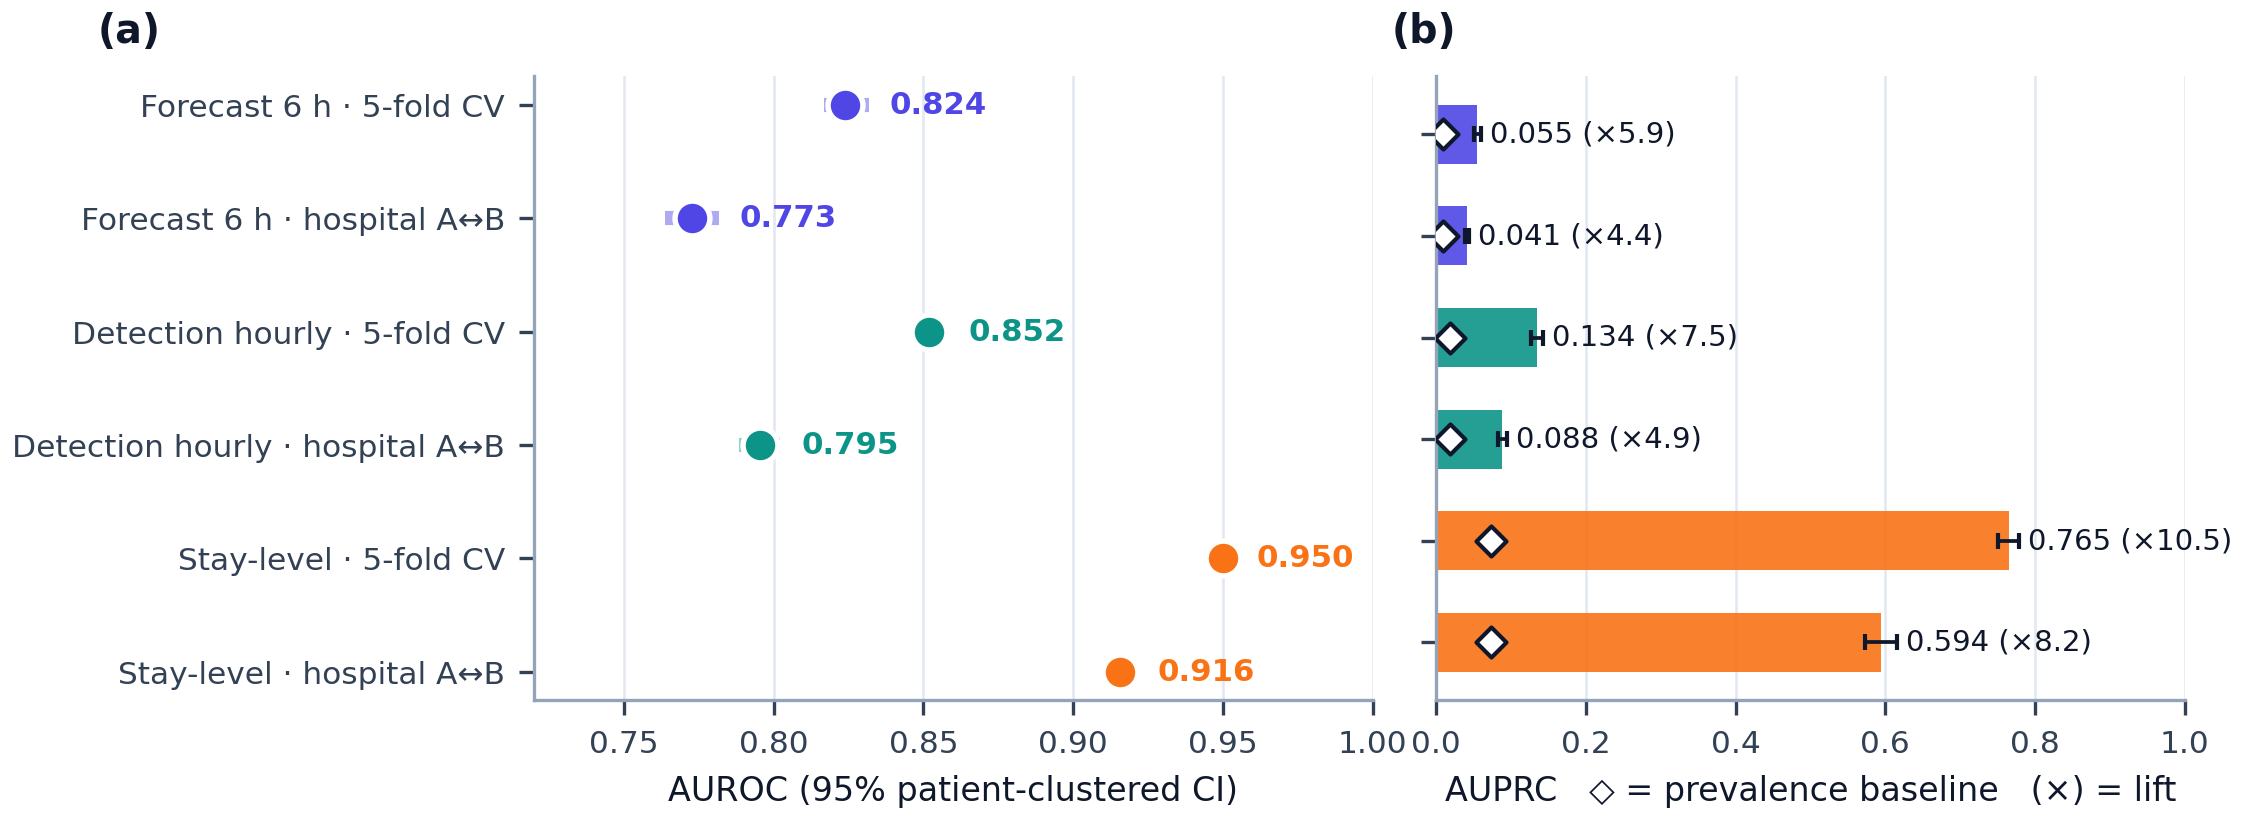
\includegraphics[width=0.892\textwidth]{figures/fig04_main_results.png}
\caption{Main results. (a) AUROC with 95\% patient-clustered intervals. (b) AUPRC against the prevalence baseline (diamond) with the lift over prevalence in brackets.}
\label{fig:main}
\end{figure*}

\begin{table*}[!t]
\centering\footnotesize
\caption{Final results at natural prevalence (pooled out-of-fold predictions; 95\% patient-clustered bootstrap CI). Patient AUROC scores each stay by its highest hourly risk.}
\label{tab:main}
\begin{adjustbox}{max width=\linewidth}
\begin{tabular}{llcccc}
\toprule
Task & Setting & AUROC [95\% CI] & AUPRC [95\% CI] & Patient AUROC & Prevalence \\
\midrule
Early prediction 6\,h & 5-fold CV & 0.824 [0.817, 0.832] & 0.055 [0.051, 0.059] & 0.795 & 0.92\% \\
Hourly detection & 5-fold CV & 0.852 [0.846, 0.858] & 0.134 [0.126, 0.143] & 0.870 & 1.80\% \\
Stay-level detection & 5-fold CV & 0.950 [0.946, 0.954] & 0.765 [0.751, 0.779] & -- & 7.27\% \\
\midrule
Early prediction 6\,h & A$\leftrightarrow$B & 0.773 [0.764, 0.782] & 0.041 [0.038, 0.044] & 0.706 & 0.92\% \\
Hourly detection & A$\leftrightarrow$B & 0.795 [0.788, 0.802] & 0.088 [0.082, 0.094] & 0.796 & 1.80\% \\
Stay-level detection & A$\leftrightarrow$B & 0.916 [0.910, 0.921] & 0.594 [0.572, 0.615] & -- & 7.27\% \\
\bottomrule
\end{tabular}
\end{adjustbox}
\end{table*}


\begin{figure}[!t]
\centering
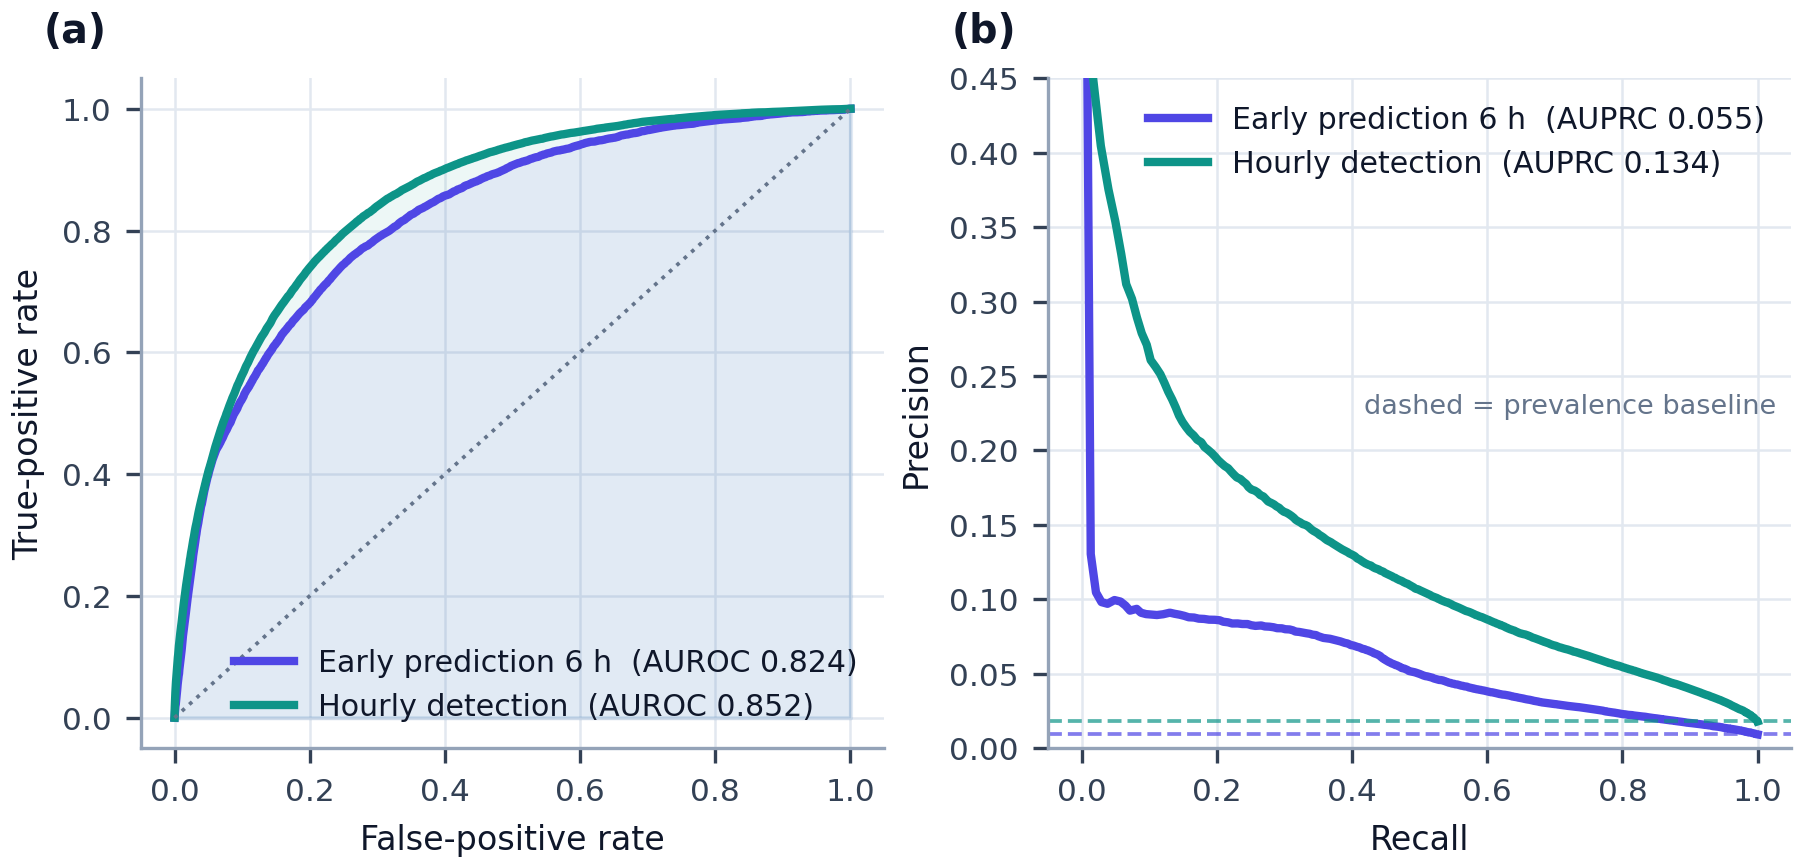
\includegraphics[width=\columnwidth]{figures/fig05_roc_pr.png}
\caption{(a) ROC and (b) precision--recall curves of the pooled out-of-fold predictions. Dashed lines in (b) show the prevalence baselines.}
\label{fig:rocpr}
\end{figure}

\subsection{Stability across folds}
Fold-to-fold variation is small (Fig.~\ref{fig:folds}, Table~\ref{tab:folds}): AUROC varies by 0.005--0.009 for the hourly tasks and by 0.006 for the stay-level task, and the AUPRC lift is similarly stable. Intervals therefore reflect sampling, not an unlucky split.

\begin{figure*}[!t]
\centering
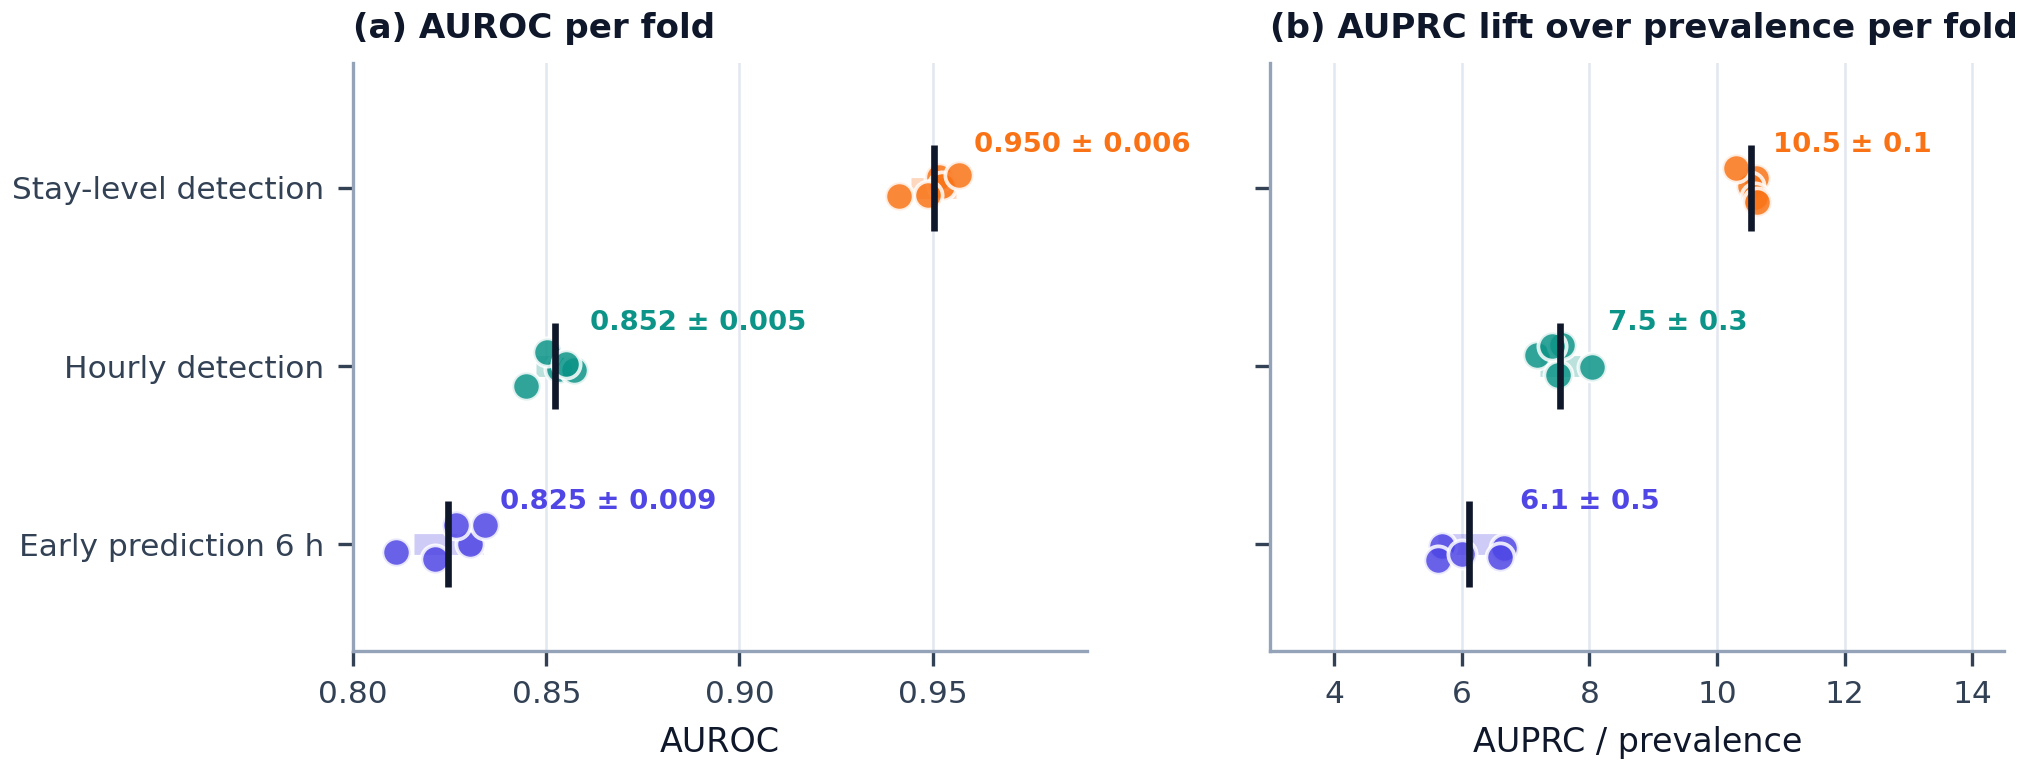
\includegraphics[width=0.874\textwidth]{figures/fig06_folds.png}
\caption{Per-fold AUROC and AUPRC lift (dots), mean (bar) and $\pm1$ SD (shaded band).}
\label{fig:folds}
\end{figure*}

\begin{table*}[!t]
\centering\footnotesize
\caption{Per-fold results (two-stage model; stay-level classifier). Folds are patient-disjoint.}
\label{tab:folds}
\begin{adjustbox}{max width=\linewidth}
\begin{tabular}{lcccccc}
\toprule
 & Forecast AUROC & Forecast AUPRC & Detect AUROC & Detect AUPRC & Stay AUROC & Stay AUPRC \\
\midrule
Fold 0 & 0.830 & 0.053 & 0.853 & 0.129 & 0.952 & 0.772 \\
Fold 1 & 0.834 & 0.051 & 0.850 & 0.135 & 0.953 & 0.764 \\
Fold 2 & 0.821 & 0.061 & 0.857 & 0.144 & 0.949 & 0.770 \\
Fold 3 & 0.827 & 0.062 & 0.855 & 0.137 & 0.957 & 0.772 \\
Fold 4 & 0.811 & 0.056 & 0.845 & 0.132 & 0.941 & 0.750 \\
\midrule
\textbf{Mean $\pm$ SD} & 0.825 $\pm$ 0.009 & 0.057 $\pm$ 0.005 & 0.852 $\pm$ 0.005 & 0.135 $\pm$ 0.006 & 0.950 $\pm$ 0.006 & 0.766 $\pm$ 0.009 \\
\bottomrule
\end{tabular}
\end{adjustbox}
\end{table*}


\subsection{Cross-hospital transfer}
Training on hospital A and testing on hospital B (and the reverse) lowers AUROC by 5.6 points for early prediction, 6.0 for hourly detection and 3.4 for stay-level detection (Fig.~\ref{fig:transfer}, Table~\ref{tab:transfer}); AUPRC for hourly detection falls from \AuprcDt{} to \AuprcDtT{}. This gap would be invisible in any single-split evaluation. Hospitals differ in prevalence (8.8\% vs 5.7\%) and, plausibly, in charting and ordering practice, which the model partly encodes (Sec.~\ref{sec:ablation}).

\begin{figure*}[!t]
\centering
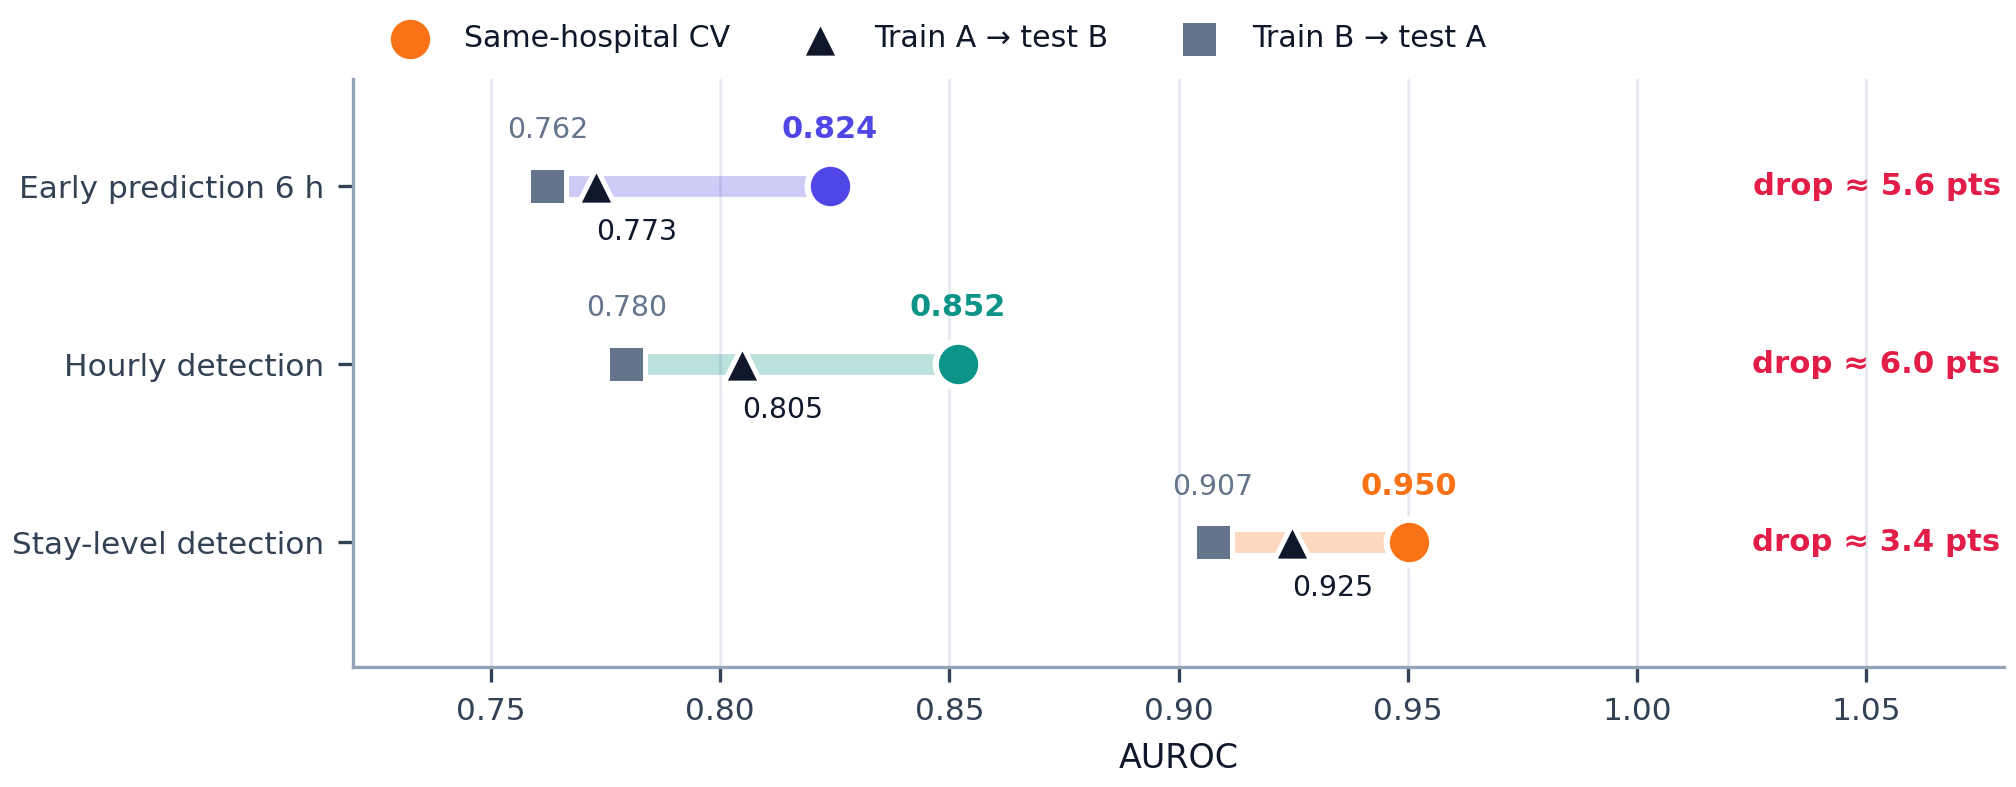
\includegraphics[width=0.828\textwidth]{figures/fig07_transfer.png}
\caption{Same-hospital cross-validation (circle) against training on A and testing on B (triangle) and the reverse (square).}
\label{fig:transfer}
\end{figure*}

\begin{table}[!t]
\centering\footnotesize\setlength{\tabcolsep}{3pt}
\caption{Cross-hospital transfer (AUROC unless stated).}
\label{tab:transfer}
\begin{adjustbox}{max width=\linewidth}
\begin{tabular}{lccccc}
\toprule
Task & CV & A$\to$B & B$\to$A & AUPRC A$\to$B & AUPRC B$\to$A \\
\midrule
Early prediction 6\,h & 0.824 & 0.773 & 0.762 & 0.033 & 0.052 \\
Hourly detection & 0.852 & 0.805 & 0.780 & 0.075 & 0.095 \\
Stay-level detection & 0.950 & 0.925 & 0.907 & 0.571 & 0.668 \\
\bottomrule
\end{tabular}
\end{adjustbox}
\end{table}


\subsection{Prediction horizon}
Lengthening the horizon does not raise AUROC (Fig.~\ref{fig:horizon}, Table~\ref{tab:horizon}): it is 0.825, 0.822 and 0.830 at 6, 12 and 24\,h. AUPRC rises from 0.060 to 0.192 only because the share of positive rows grows from 0.92\% to 3.08\%; the lift over prevalence actually falls from 6.5 to 6.2. Horizon alone is therefore not a route to better discrimination.

\begin{figure}[!t]
\centering
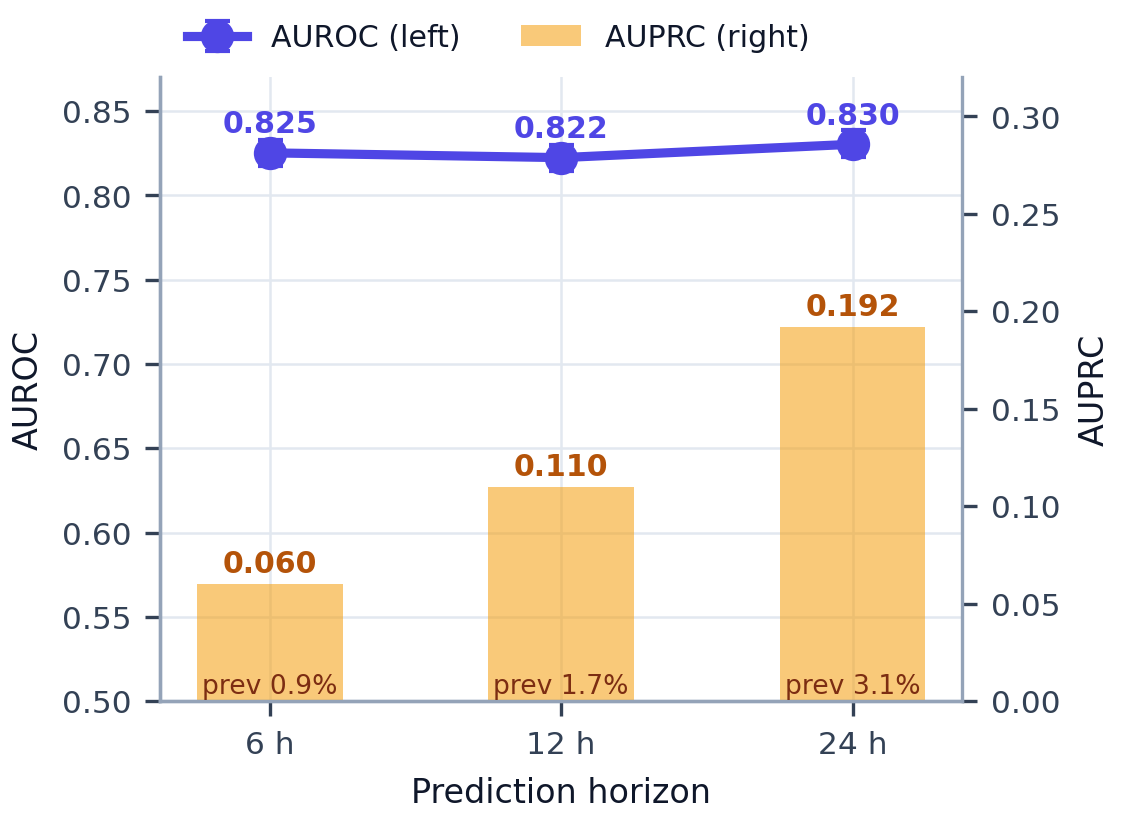
\includegraphics[width=\columnwidth]{figures/fig08_horizon.png}
\caption{AUROC (line, left) and AUPRC (bars, right) for 6, 12 and 24\,h horizons.}
\label{fig:horizon}
\end{figure}

\begin{table}[!t]
\centering\footnotesize\setlength{\tabcolsep}{3pt}
\caption{Prediction horizon (single-stage boosted model, 5-fold CV). AUPRC rises with the horizon only because more rows are positive.}
\label{tab:horizon}
\begin{adjustbox}{max width=\linewidth}
\begin{tabular}{lcccc}
\toprule
Horizon & AUROC [95\% CI] & AUPRC [95\% CI] & Prev. & Lift \\
\midrule
6\,h & 0.825 [0.817, 0.833] & 0.060 [0.055, 0.065] & 0.92\% & $\times$6.5 \\
12\,h & 0.822 [0.814, 0.830] & 0.110 [0.103, 0.118] & 1.73\% & $\times$6.4 \\
24\,h & 0.830 [0.823, 0.839] & 0.192 [0.180, 0.204] & 3.08\% & $\times$6.2 \\
\bottomrule
\end{tabular}
\end{adjustbox}
\end{table}


\subsection{Care-process shortcuts}
\label{sec:ablation}
Gain importance is dominated by measurement-timing features (53\% of top-15 gain for early prediction) and care-pathway variables (35\%), led by ICULOS (Fig.~\ref{fig:importance}). Such features describe clinical workflow as much as physiology. Removing ICULOS, admission time and unit lowers AUROC by only 0.005--0.006; also removing measurement timing lowers it by 0.026 (forecast) and 0.027 (detection) within a hospital, and by 0.041 and 0.033 across hospitals (Fig.~\ref{fig:ablation}, Table~\ref{tab:ablation}). The model still discriminates from physiology alone, but part of its score reflects \emph{how often} a patient is measured. This is a limitation for deployment, where charting practice changes.

\begin{figure*}[!t]
\centering
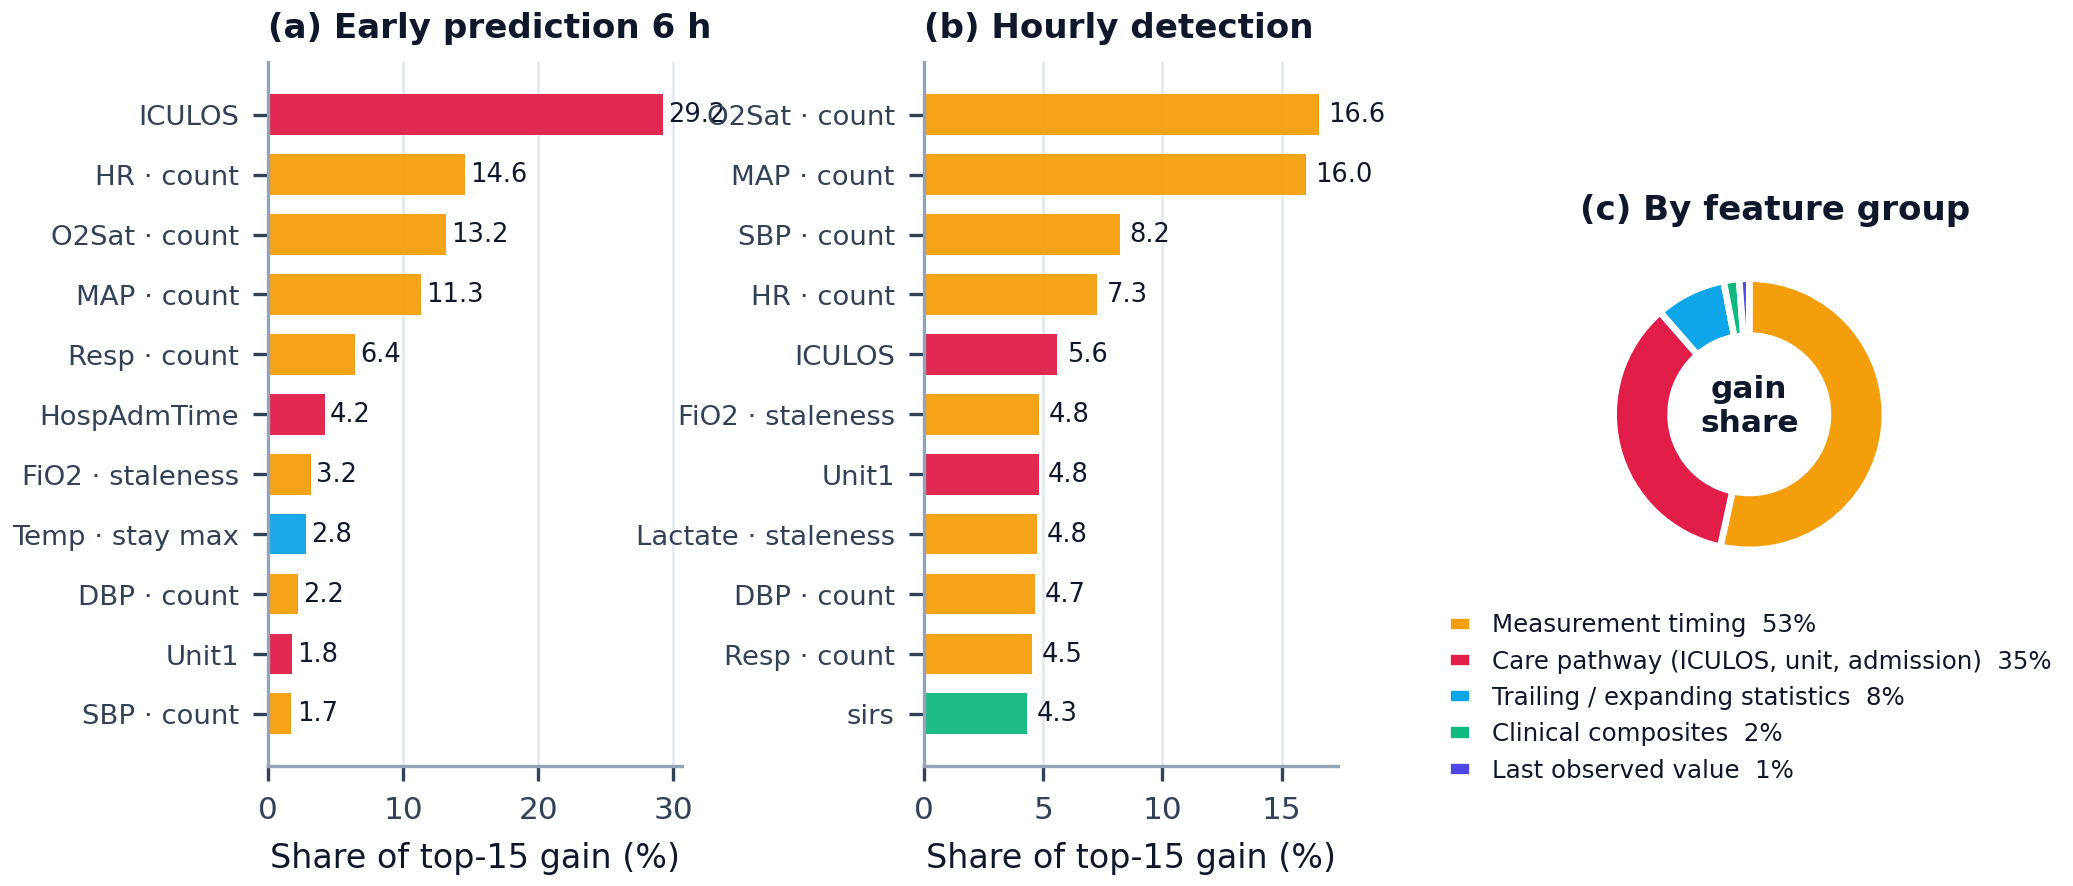
\includegraphics[width=0.892\textwidth]{figures/fig10_importance.png}
\caption{Gain importance of the single-stage boosted model (mean over folds; top-15 per fold). Colors give the feature group. (c) Group share of gain for early prediction.}
\label{fig:importance}
\end{figure*}

\begin{figure*}[!t]
\centering
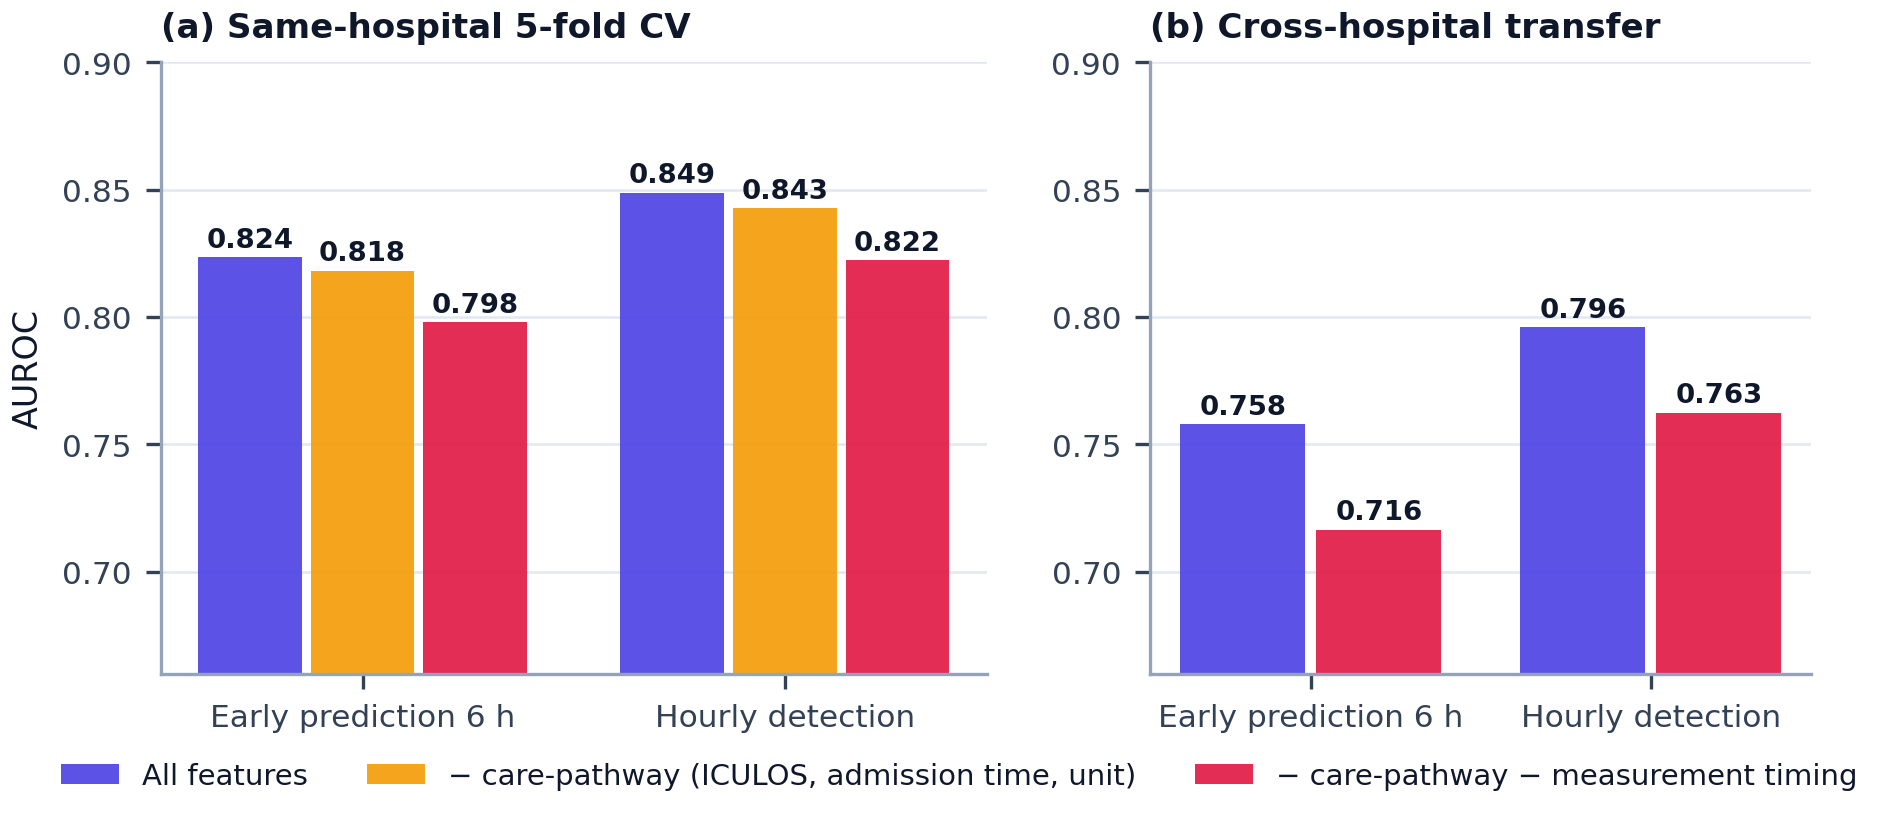
\includegraphics[width=0.856\textwidth]{figures/fig09_ablation.png}
\caption{Shortcut ablation. Removing care-pathway variables costs little; removing measurement timing as well costs more, especially across hospitals.}
\label{fig:ablation}
\end{figure*}

\begin{table}[!t]
\centering\footnotesize\setlength{\tabcolsep}{3pt}
\caption{Shortcut ablation (AUROC, boosted model). ``No care'' drops ICULOS/admission time/unit; ``physio-only'' also drops all measurement-timing features.}
\label{tab:ablation}
\begin{adjustbox}{max width=\linewidth}
\begin{tabular}{llcccc}
\toprule
Task & Setting & All & No care & Physio-only & $\Delta$ \\
\midrule
Early 6\,h & CV & 0.824 & 0.818 & 0.798 & -0.026 \\
Early 6\,h & A$\leftrightarrow$B & 0.758 & -- & 0.716 & -0.041 \\
Detection & CV & 0.849 & 0.843 & 0.822 & -0.026 \\
Detection & A$\leftrightarrow$B & 0.796 & -- & 0.763 & -0.033 \\
\bottomrule
\end{tabular}
\end{adjustbox}
\end{table}


\subsection{Calibration and lead time}
After cross-fold isotonic calibration the predicted risks track the observed event rates over two orders of magnitude (ECE 0.0003 and 0.0001; Fig.~\ref{fig:calib}), and Brier scores improve on constant-prevalence prediction by 2.7\% and 6.5\%. Skill is modest because events are rare, but the probabilities are usable. As an illustrative operating-point analysis, if a threshold is set so that 10, 20 or 30\% of non-septic stays raise an alert at some point, then 48, 57 and 65\% of septic stays are alerted at least 6\,h before the first positive label (Fig.~\ref{fig:lead}); thresholds here are set on the pooled out-of-fold scores and are not a validated deployment rule. Table~\ref{tab:operating} gives row-level operating points: at 90\% specificity the early-prediction model detects 52\% of positive rows with 21.5 alerts per true positive, and the detection model 56\% with 10.7.

\begin{figure*}[!t]
\centering
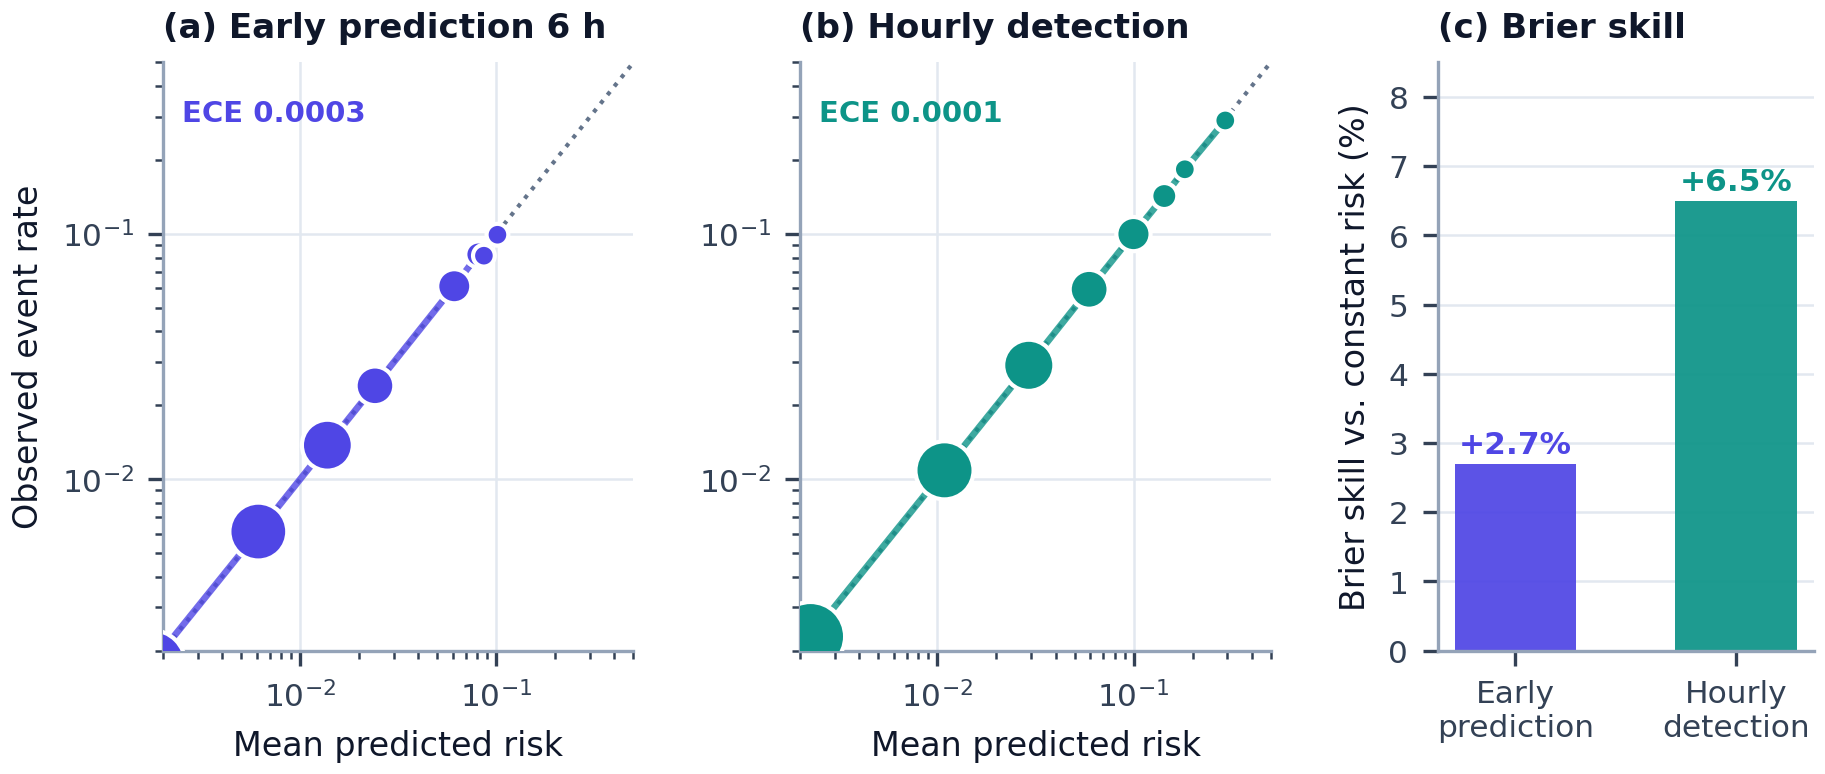
\includegraphics[width=0.874\textwidth]{figures/fig11_calibration.png}
\caption{Reliability of the calibrated risk for (a) early prediction and (b) detection on log--log axes (marker area $\propto\sqrt{n}$); (c) Brier skill over constant-prevalence prediction.}
\label{fig:calib}
\end{figure*}

\begin{table}[!t]
\centering\scriptsize
\caption{Row-level operating points of the final model (pooled out-of-fold; threshold set on the same predictions, so illustrative). A/TP = alerts per true positive.}
\label{tab:operating}
\begin{adjustbox}{max width=\linewidth}
\begin{tabular}{lcccc}
\toprule
Task & Specificity & Sensitivity & Precision & A/TP \\
\midrule
Early 6\,h & 90\% & 0.523 & 0.047 & 21.5 \\
Early 6\,h & 95\% & 0.399 & 0.069 & 14.4 \\
Early 6\,h & 99\% & 0.105 & 0.089 & 11.2 \\
\midrule
Detection & 90\% & 0.563 & 0.093 & 10.7 \\
Detection & 95\% & 0.404 & 0.129 & 7.8 \\
Detection & 99\% & 0.152 & 0.217 & 4.6 \\
\bottomrule
\end{tabular}
\end{adjustbox}
\end{table}


\begin{figure}[!t]
\centering
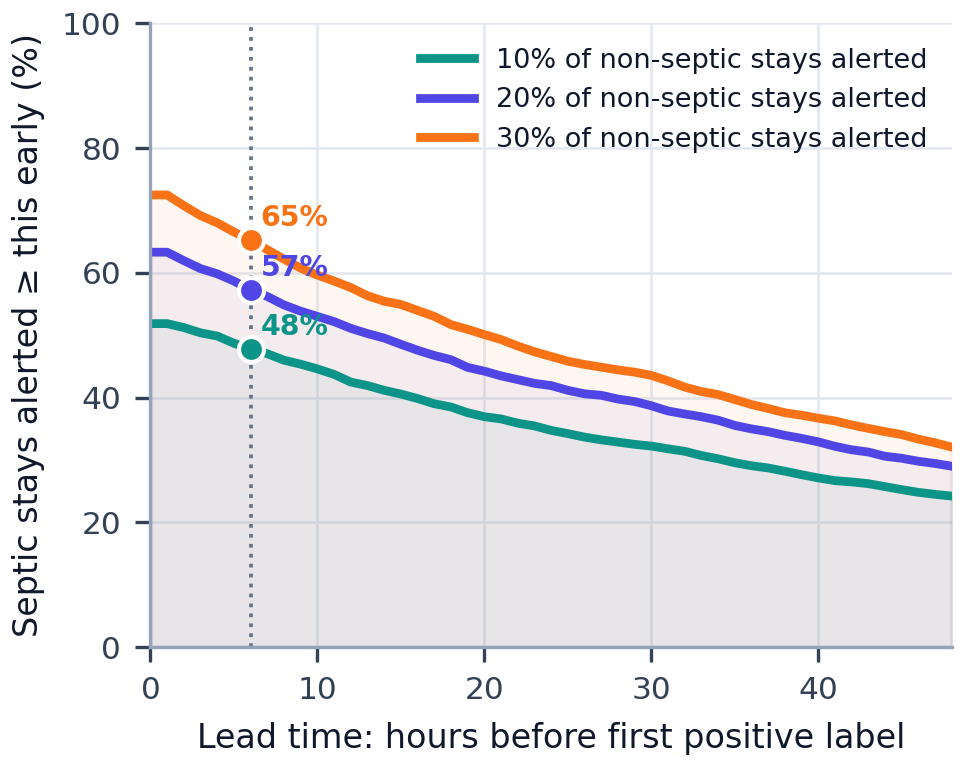
\includegraphics[width=\columnwidth]{figures/fig12_leadtime.png}
\caption{Fraction of septic stays alerted at least a given number of hours before the first positive label, for three false-alert budgets (early prediction, pooled out-of-fold scores).}
\label{fig:lead}
\end{figure}

\textbf{Calibration across hospitals.} Calibration degrades when the model is applied to the other hospital (Table~\ref{tab:transcal}). Here we evaluate the uncalibrated second-stage probability in all three settings, because no recalibration on the target hospital is allowed. For early prediction the observed-to-expected ratio is 0.99 within hospital, 0.75 for A$\to$B (over-prediction) and 1.22 for B$\to$A (under-prediction), the direction expected from the prevalence difference between the hospitals (8.8\% vs 5.7\% septic stays), and ECE is 4--5 times its within-hospital value (0.0023--0.0028 vs 0.0006). For hourly detection both directions over-predict (O/E 0.95 and 0.82) and ECE rises from 0.0010 to 0.0035--0.0069, so prevalence shift alone does not explain it. Calibration slopes of 0.77--0.91 indicate over-confident scores, and the A$\to$B early-prediction Brier skill ($-0.3$\%) is no better than constant-prevalence prediction. Recalibration to the local prevalence would be needed before use at a new site.

\begin{table}[!t]
\centering\footnotesize\setlength{\tabcolsep}{4pt}
\caption{Calibration of the uncalibrated second-stage probability within hospital and across hospitals. O/E: observed over expected events ($<1$ over-prediction); slope: logistic calibration slope (1 is ideal); ECE: expected calibration error (20 quantile bins); BSS: Brier skill over constant-prevalence prediction.}
\label{tab:transcal}
\begin{tabular}{llcccc}
\toprule
Task & Setting & O/E & Slope & ECE & BSS \\
\midrule
Early 6\,h & Within-hospital CV & 0.99 & 0.96 & 0.0006 & 2.7\% \\
 & A$\to$B & 0.75 & 0.77 & 0.0028 & $-0.3$\% \\
 & B$\to$A & 1.22 & 0.91 & 0.0023 & 2.1\% \\
\midrule
Detection & Within-hospital CV & 1.02 & 1.04 & 0.0010 & 6.6\% \\
 & A$\to$B & 0.95 & 0.82 & 0.0035 & 2.4\% \\
 & B$\to$A & 0.82 & 0.77 & 0.0069 & 2.2\% \\
\bottomrule
\end{tabular}
\end{table}

\subsection{Subgroups, decision curves and alert burden}
\textbf{Subgroups.} Discrimination is similar across subgroups (Table~\ref{tab:subgroups}). For early prediction, AUROC ranges from 0.813 (age $\geq$80) to 0.830 (age $<$45) across age bands and is 0.823 for female and 0.825 for male patients; for hourly detection the corresponding ranges are 0.846--0.857 across age bands and 0.849--0.855 across sexes. The 95\% intervals of the age bands overlap. The hospitals differ more: for early prediction hospital B is slightly lower (0.813 vs 0.822, overlapping intervals), whereas for hourly detection hospital B is higher (0.869 vs 0.832, non-overlapping intervals), alongside its lower row prevalence (1.4\% vs 2.2\%).

\textbf{Decision curves.} At a threshold probability of 1\%, the net benefit of early prediction is 4.3 per 1000 rows against $-0.8$ for alerting on every row, and for hourly detection 12.3 against 8.1 (Fig.~\ref{fig:dca}). The model exceeds both defaults over the plotted range for hourly detection and up to about 0.11 for early prediction, although the early-prediction net benefit is close to zero above about 0.09 because few rows receive such a high predicted risk. The analysis is at row level and assumes no particular cost of a false alarm.

\textbf{Alert burden.} At 90\% row-level specificity, the early-prediction model raises 2.4 false alarms per patient-day and 21.5 alerts per true positive, and alerts 59\% of septic stays before the first positive label with a median lead of 42\,h (IQR 16--85); at 95\% specificity false alarms halve to 1.2 per patient-day and 43\% of septic stays are alerted (Table~\ref{tab:burden}). This lead time is measured from the first alert anywhere in the stay and so includes isolated early alerts; it is not a time to a sustained alert.

\begin{figure}[!t]
\centering
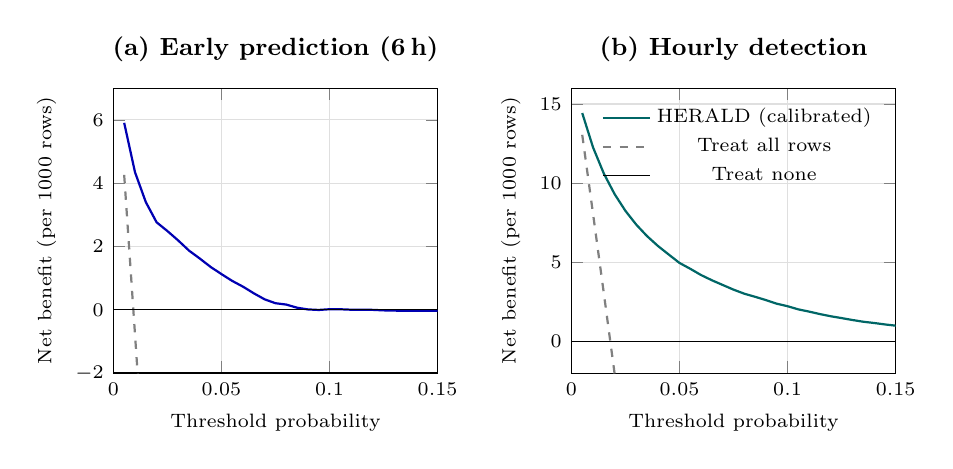
\begin{tikzpicture}
\begin{groupplot}[group style={group size=2 by 1, horizontal sep=1.7cm}, width=0.47\textwidth, height=5.2cm, xmin=0, xmax=0.15,
 xlabel={Threshold probability}, ylabel={Net benefit (per 1000 rows)}, grid=major, grid style={gray!25}, tick label style={font=\scriptsize}, label style={font=\scriptsize},
 xtick={0,0.05,0.1,0.15}, scaled x ticks=false, xticklabel style={/pgf/number format/fixed}, title style={font=\small\bfseries}, legend style={font=\scriptsize, draw=none, fill=none}]
\nextgroupplot[title={(a) Early prediction (6\,h)}, ymin=-2, ymax=7]
\addplot[blue!70!black, thick] coordinates {(0.005,5.904) (0.010,4.345) (0.015,3.401) (0.020,2.761) (0.025,2.485) (0.030,2.187) (0.035,1.867) (0.040,1.616) (0.045,1.351) (0.050,1.125) (0.055,0.909) (0.060,0.727) (0.065,0.517) (0.070,0.327) (0.075,0.205) (0.080,0.162) (0.085,0.063) (0.090,0.009) (0.095,-0.008) (0.100,0.015) (0.105,0.014) (0.110,0.000) (0.115,-0.000) (0.120,-0.005) (0.125,-0.021) (0.130,-0.029) (0.135,-0.032) (0.140,-0.033) (0.145,-0.034) (0.150,-0.036)};
\addplot[gray, dashed, thick] coordinates {(0.005,4.258) (0.010,-0.771) (0.015,-5.851) (0.020,-10.983) (0.025,-16.168) (0.030,-21.406) (0.035,-26.698) (0.040,-32.045) (0.045,-37.449) (0.050,-42.909) (0.055,-48.427) (0.060,-54.004) (0.065,-59.640) (0.070,-65.337) (0.075,-71.096) (0.080,-76.917) (0.085,-82.802) (0.090,-88.751) (0.095,-94.766) (0.100,-100.848) (0.105,-106.998) (0.110,-113.218) (0.115,-119.507) (0.120,-125.868) (0.125,-132.301) (0.130,-138.809) (0.135,-145.391) (0.140,-152.051) (0.145,-158.788) (0.150,-165.604)};
\addplot[black, thin] coordinates {(0,0) (0.15,0)};
\nextgroupplot[title={(b) Hourly detection}, ymin=-2, ymax=16, legend pos=north east]
\addplot[teal!80!black, thick] coordinates {(0.005,14.428) (0.010,12.257) (0.015,10.603) (0.020,9.300) (0.025,8.245) (0.030,7.377) (0.035,6.650) (0.040,6.033) (0.045,5.491) (0.050,4.957) (0.055,4.587) (0.060,4.191) (0.065,3.862) (0.070,3.565) (0.075,3.270) (0.080,3.013) (0.085,2.818) (0.090,2.610) (0.095,2.383) (0.100,2.223) (0.105,2.023) (0.110,1.882) (0.115,1.725) (0.120,1.589) (0.125,1.473) (0.130,1.353) (0.135,1.243) (0.140,1.164) (0.145,1.073) (0.150,0.995)};
\addplot[gray, dashed, thick] coordinates {(0.005,13.050) (0.010,8.065) (0.015,3.030) (0.020,-2.056) (0.025,-7.195) (0.030,-12.387) (0.035,-17.632) (0.040,-22.933) (0.045,-28.288) (0.050,-33.700) (0.055,-39.170) (0.060,-44.697) (0.065,-50.284) (0.070,-55.930) (0.075,-61.638) (0.080,-67.408) (0.085,-73.241) (0.090,-79.138) (0.095,-85.100) (0.100,-91.128) (0.105,-97.224) (0.110,-103.388) (0.115,-109.622) (0.120,-115.927) (0.125,-122.303) (0.130,-128.753) (0.135,-135.278) (0.140,-141.878) (0.145,-148.556) (0.150,-155.312)};
\addplot[black, thin] coordinates {(0,0) (0.15,0)};
\legend{HERALD (calibrated), Treat all rows, Treat none}
\end{groupplot}
\end{tikzpicture}
\caption{Decision curves of the final model: net benefit per 1000 rows against threshold probability, with the defaults of alerting on every row (dashed) and on none (zero line). Risks are calibrated by cross-fold isotonic regression.}
\label{fig:dca}
\end{figure}

\begin{table}[!t]
\centering\scriptsize\setlength{\tabcolsep}{3pt}
\caption{Subgroup performance of the final model (pooled out-of-fold, natural prevalence). AUROC with 95\% patient-clustered bootstrap intervals (300 replicates); AUPRC is a point estimate and lift is AUPRC over the subgroup's own prevalence. Age bands in years; sex as coded in the challenge data.}
\label{tab:subgroups}
\begin{adjustbox}{max width=\linewidth}
\begin{tabular}{llcrcccc}
\toprule
Task & Group & Level & Patients & Prev.\ (\%) & AUROC [95\% CI] & AUPRC & Lift \\
\midrule
Early 6 h & Age (years) & $<$45 & 6{,}315 & 0.92 & 0.830 [0.811, 0.851] & 0.062 & 6.7 \\
 &  & 45--64 & 14{,}856 & 0.90 & 0.825 [0.812, 0.838] & 0.053 & 5.9 \\
 &  & 65--79 & 13{,}430 & 0.96 & 0.824 [0.812, 0.837] & 0.056 & 5.8 \\
 &  & $\geq$80 & 5{,}309 & 0.89 & 0.813 [0.789, 0.834] & 0.053 & 6.0 \\
 & Sex & Female & 17{,}595 & 0.85 & 0.823 [0.810, 0.836] & 0.055 & 6.5 \\
 &  & Male & 22{,}315 & 0.98 & 0.825 [0.814, 0.834] & 0.055 & 5.6 \\
 & Hospital & A & 20{,}133 & 1.15 & 0.822 [0.814, 0.832] & 0.063 & 5.5 \\
 &  & B & 19{,}777 & 0.69 & 0.813 [0.799, 0.828] & 0.041 & 5.9 \\
\midrule
Detection & Age (years) & $<$45 & 6{,}388 & 1.84 & 0.857 [0.842, 0.871] & 0.143 & 7.8 \\
 &  & 45--64 & 15{,}024 & 1.78 & 0.852 [0.844, 0.862] & 0.138 & 7.8 \\
 &  & 65--79 & 13{,}557 & 1.83 & 0.851 [0.841, 0.860] & 0.133 & 7.3 \\
 &  & $\geq$80 & 5{,}367 & 1.74 & 0.846 [0.830, 0.863] & 0.122 & 7.0 \\
 & Sex & Female & 17{,}770 & 1.66 & 0.855 [0.846, 0.864] & 0.133 & 8.0 \\
 &  & Male & 22{,}566 & 1.91 & 0.849 [0.842, 0.858] & 0.135 & 7.1 \\
 & Hospital & A & 20{,}336 & 2.17 & 0.832 [0.824, 0.840] & 0.127 & 5.8 \\
 &  & B & 20{,}000 & 1.41 & 0.869 [0.860, 0.877] & 0.145 & 10.3 \\
\bottomrule
\end{tabular}
\end{adjustbox}
\end{table}

\begin{table}[!t]
\centering\scriptsize
\caption{Alert burden at fixed row-level specificity (pooled out-of-fold; thresholds set on the same predictions, so illustrative). False alarms are alerts on rows with a negative target per 24 patient-hours. Lead time is the time from the first alert to the first positive label, median [IQR] over septic stays alerted before the label.}
\label{tab:burden}
\begin{adjustbox}{max width=\linewidth}
\begin{tabular}{lccccc}
\toprule
Task & Spec. & False alarms / patient-day & Alerts / TP & Septic stays alerted & Lead time (h) \\
\midrule
Early 6 h & 90\% & 2.38 & 21.5 & 59\% & 42 [16--85] \\
Early 6 h & 95\% & 1.19 & 14.4 & 43\% & 43 [17--85] \\
Detection & 90\% & 2.36 & 10.7 & 57\% & 40 [14--83] \\
Detection & 95\% & 1.18 & 7.8 & 44\% & 40 [14--86] \\
\bottomrule
\end{tabular}
\end{adjustbox}
\end{table}

\subsection{Stay-level detection}
Scoring whole stays retrospectively gives AUROC \AurocStay{} and AUPRC \AuprcStay{} (prevalence 7.27\%), and \AurocStayT{} and \AuprcStayT{} across hospitals (Fig.~\ref{fig:stay}). Because septic stays could simply be longer, we checked three things. Stay length alone gives AUROC only \LenAlone; the model's AUROC within each length quartile is 0.88--0.96; and the primary variant uses no length, ICULOS or timing features. On a balanced 432/432 view the same predictions give AUROC \BalAuroc{} and AUPRC \BalAuprc{}, which illustrates how strongly AUPRC depends on the test prevalence. This task uses the whole stay, including post-onset hours, and must not be read as early warning.

\begin{figure*}[!t]
\centering
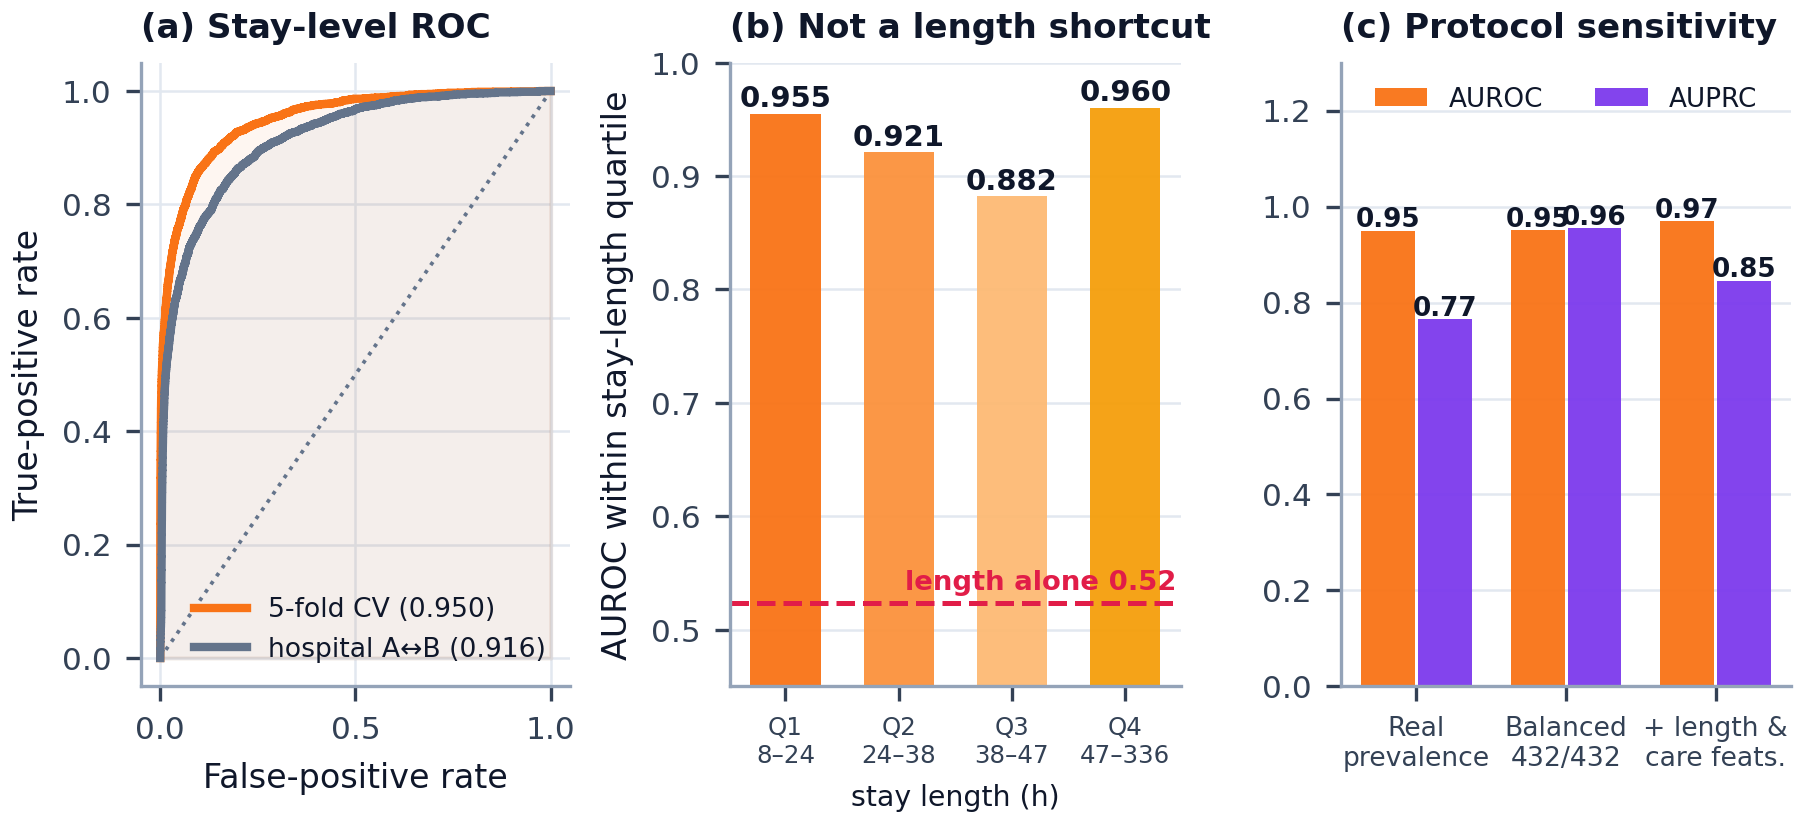
\includegraphics[width=0.892\textwidth]{figures/fig13_stay_level.png}
\caption{Stay-level detection. (a) ROC curves. (b) AUROC within stay-length quartiles, with the AUROC of stay length alone (dashed). (c) The same predictions under three protocols.}
\label{fig:stay}
\end{figure*}

\subsection{Model families and negative results}
A causal TCN reached AUROC 0.803 (forecast) and 0.820 (detection), below boosting, and averaging it with the boosted model did not help (Fig.~\ref{fig:family}, Table~\ref{tab:family}); we therefore dropped it from the final model. The second stage changes AUROC by $-0.001$ for early prediction and $+0.002$ for detection and lowers early-prediction AUPRC from 0.060 to 0.055 (Table~\ref{tab:stage}); all differences lie within the bootstrap intervals, so stacking adds little. We keep the two-stage model as the final model because that design was fixed before test results were examined. On validation patients only, personal-baseline features, a multi-horizon soft label, positive-class weighting and a three-configuration average all failed a pre-set adoption rule (Fig.~\ref{fig:negative}, Table~\ref{tab:negative}). The consistent picture is that the information in this dataset, not the learner, limits performance at roughly 0.82--0.85 AUROC for hourly tasks.

\begin{figure*}[!t]
\centering
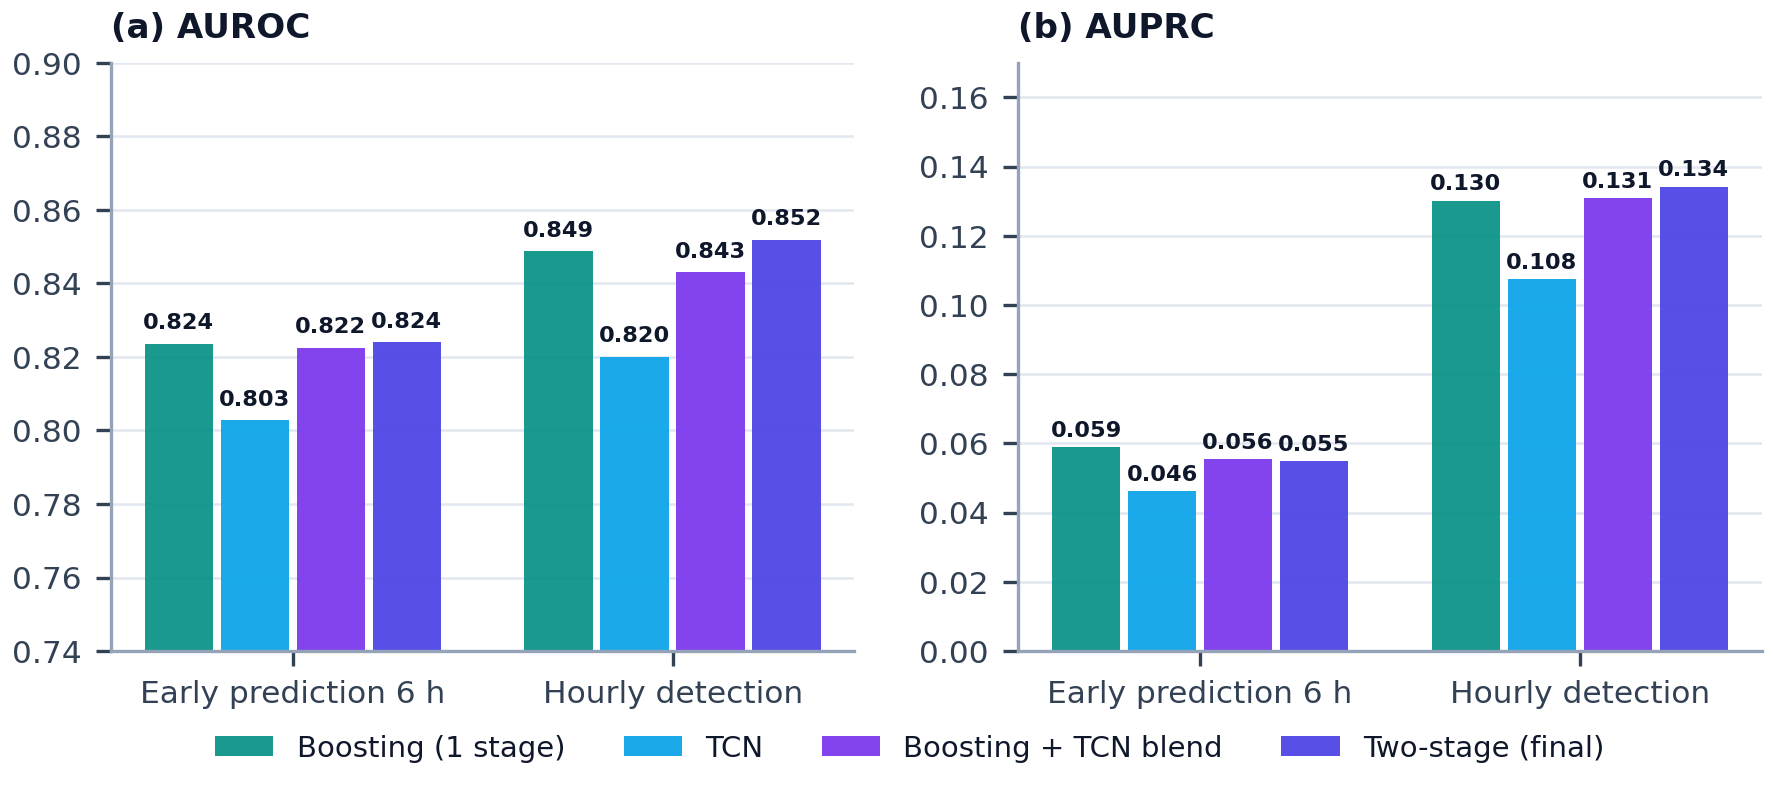
\includegraphics[width=0.856\textwidth]{figures/fig18_model_family.png}
\caption{Model families on 5-fold cross-validation: single-stage boosting, TCN, their blend and the two-stage final model.}
\label{fig:family}
\end{figure*}

\begin{figure}[!t]
\centering
\includegraphics[width=\columnwidth]{fig17_negative_results.png}
\caption{Validation-only change in AUROC for ideas tested; the dashed line is the adoption threshold. Only the 306$\to$370 feature extension passed.}
\label{fig:negative}
\end{figure}

\begin{table*}[!t]
\centering\footnotesize
\caption{Model families (5-fold CV, pooled). The TCN did not improve on boosting.}
\label{tab:family}
\begin{adjustbox}{max width=\linewidth}
\begin{tabular}{llcc}
\toprule
Task & Model & AUROC [95\% CI] & AUPRC [95\% CI] \\
\midrule
Early 6\,h & Boosting (1 stage) & 0.824 [0.816, 0.831] & 0.059 [0.055, 0.063] \\
Early 6\,h & TCN & 0.803 [0.795, 0.811] & 0.046 [0.044, 0.049] \\
Early 6\,h & Boosting + TCN blend & 0.822 [0.815, 0.830] & 0.056 [0.052, 0.060] \\
Early 6\,h & Two-stage (final) & 0.824 [0.817, 0.832] & 0.055 [0.051, 0.059] \\
\midrule
Detection & Boosting (1 stage) & 0.849 [0.843, 0.854] & 0.130 [0.122, 0.139] \\
Detection & TCN & 0.820 [0.814, 0.826] & 0.108 [0.101, 0.115] \\
Detection & Boosting + TCN blend & 0.843 [0.837, 0.849] & 0.131 [0.123, 0.140] \\
Detection & Two-stage (final) & 0.852 [0.846, 0.858] & 0.134 [0.126, 0.143] \\
\bottomrule
\end{tabular}
\end{adjustbox}
\end{table*}

\begin{table}[!t]
\centering\scriptsize
\caption{Value of the second stage (5-fold CV, pooled). It changes AUROC by $-0.001$ (forecast) and $+0.002$ (detection).}
\label{tab:stage}
\begin{adjustbox}{max width=\linewidth}
\begin{tabular}{llcc}
\toprule
Task & Model & AUROC [95\% CI] & AUPRC [95\% CI] \\
\midrule
Early 6\,h & Stage 1 only & 0.825 [0.817, 0.833] & 0.060 [0.055, 0.065] \\
Early 6\,h & Stage 1 + 2 (final) & 0.824 [0.817, 0.832] & 0.055 [0.051, 0.059] \\
\midrule
Detection & Stage 1 only & 0.850 [0.845, 0.856] & 0.132 [0.124, 0.141] \\
Detection & Stage 1 + 2 (final) & 0.852 [0.846, 0.858] & 0.134 [0.126, 0.143] \\
\bottomrule
\end{tabular}
\end{adjustbox}
\end{table}

\begin{table}[!t]
\centering\footnotesize\setlength{\tabcolsep}{3pt}
\caption{Ideas tested on validation patients only (change vs.\ the 370-feature set). None met the pre-set adoption rule ($\Delta$AUROC $\ge +0.001$ and AUPRC not down $>3\%$).}
\label{tab:negative}
\begin{adjustbox}{max width=\linewidth}
\begin{tabular}{llcc}
\toprule
Task & Idea & $\Delta$ val AUROC & $\Delta$ val AUPRC \\
\midrule
Early 6\,h & Personal-baseline features & -0.0039 & +5.4\% \\
Early 6\,h & Multi-horizon soft label & -0.0014 & -5.4\% \\
Early 6\,h & Positive weight $\times$3 & -0.0230 & -12.0\% \\
Early 6\,h & Mean of 3 configurations & -0.0011 & +2.7\% \\
\midrule
Detection & Personal-baseline features & -0.0030 & +5.0\% \\
Detection & Positive weight $\times$3 & -0.0129 & -9.3\% \\
Detection & Mean of 3 configurations & -0.0002 & +5.4\% \\
\bottomrule
\end{tabular}
\end{adjustbox}
\end{table}


\section{Multi-Criteria Evaluation with TOPSIS}
\label{sec:topsis}
\subsection{Method}
\label{sec:topsis_method}
TOPSIS ranks alternatives by their distance to an ideal solution \cite{hwang1981}; \cite{behzadian2012} surveys its applications. Given a decision matrix $x_{ij}$ of $m$ alternatives and $n$ criteria, we normalize $r_{ij}=x_{ij}/\sqrt{\sum_i x_{ij}^2}$, weight $v_{ij}=w_j r_{ij}$ with $\sum_j w_j=1$, and compute distances $d_i^{\pm}$ to the positive and negative ideal points. The closeness
\begin{equation}
C_i^{*}=\frac{d_i^{-}}{d_i^{+}+d_i^{-}}\in[0,1]
\end{equation}
is larger for alternatives closer to the ideal. Weights are a judgement; we therefore always show several weightings.

\subsection{Earlier baseline models on identical patients}
We scored \herald{} and the earlier baseline models on exactly the same 229{,}244 forecast rows (5{,}983 test patients) with one code path, using AUROC, AUPRC, patient AUROC, sensitivity at 90\% specificity and alerts per true positive (a cost criterion). \herald{} ranks first (C$^*$ \TopsisV{} vs.\ \TopsisL{} for the best earlier LightGBM) under all four weightings (Fig.~\ref{fig:topsis_models}, Fig.~\ref{fig:topsis_sens}, Table~\ref{tab:topsis_models}). The margin is small: AUPRC is nearly tied (0.0513 vs.\ 0.0510), and the earlier LightGBM is slightly ahead on patient AUROC and sensitivity. \herald{} was trained on 80\% of all patients in cross-validation, whereas the earlier models used 60\%, which slightly favors \herald{}.

\begin{figure*}[!t]
\centering
\includegraphics[width=0.874\textwidth]{fig14_topsis_models.png}
\caption{(a) TOPSIS closeness (equal weights) of the models on identical rows. (b) Radar of min--max normalized criteria for the three most informative models.}
\label{fig:topsis_models}
\end{figure*}

\begin{table*}[!t]
\centering\footnotesize\setlength{\tabcolsep}{3.4pt}
\caption{TOPSIS on the \emph{identical} 229{,}244 forecast rows (5{,}983 test patients) of the earlier baseline models: criteria and closeness $C^*$ under four weightings. Equal weights are used because the original weights were not archived; AlertsPerTP is a cost criterion. \herald{} was trained on 80\% of patients per fold and the earlier models on 60\%, which slightly favors \herald{}.}
\label{tab:topsis_models}
\begin{adjustbox}{max width=\linewidth}
\begin{tabular}{lccccccccc}
\toprule
Model & AUROC & AUPRC & PatAUROC & Sens@90 & A/TP & $C^*$ eq. & AUROC-hvy & AUPRC-hvy & Op.pt-hvy \\
\midrule
HERALD (ours) & 0.817 & 0.051 & 0.788 & 0.500 & 22.9 & 0.992 & 0.993 & 0.997 & 0.990 \\
LightGBM & 0.810 & 0.051 & 0.790 & 0.500 & 22.8 & 0.967 & 0.936 & 0.975 & 0.979 \\
LightGBM-reg & 0.811 & 0.046 & 0.789 & 0.495 & 23.1 & 0.663 & 0.708 & 0.612 & 0.774 \\
LightGBM no-meas. & 0.807 & 0.043 & 0.775 & 0.493 & 23.2 & 0.489 & 0.561 & 0.402 & 0.669 \\
Causal encoder & 0.756 & 0.041 & 0.731 & 0.459 & 24.8 & 0.179 & 0.152 & 0.204 & 0.116 \\
Causal enc.+aux & 0.771 & 0.038 & 0.737 & 0.457 & 24.9 & 0.059 & 0.126 & 0.025 & 0.037 \\
\bottomrule
\end{tabular}
\end{adjustbox}
\end{table*}


\begin{figure}[!t]
\centering
\includegraphics[width=\columnwidth]{fig15_topsis_sensitivity.png}
\caption{TOPSIS closeness of the models on identical rows under four weightings; \herald{} ranks first in all of them.}
\label{fig:topsis_sens}
\end{figure}

\subsection{Where this work is stronger, and where it is not}
\textbf{Stronger:} (i) an end-to-end leakage audit with a negative control; (ii) natural-prevalence, patient-level evaluation with bootstrap intervals; (iii) cross-hospital transfer; (iv) shortcut ablations and disclosed negative results; (v) calibrated outputs and one model family for early prediction, detection and stay-level scoring. \textbf{Not stronger:} (i) absolute scores are not above the best published ones (0.95 on a balanced patient-level test set; 0.99 on matched eICU cohorts), although those are not comparable protocols; (ii) the margin over a tuned LightGBM is small; (iii) there is no independent external dataset; (iv) a large share of the signal is measurement timing. We therefore claim comparable discrimination under a stricter, audited protocol, not state-of-the-art accuracy.

\section{Discussion}
\textbf{Why scores plateau.} Boosting, a temporal CNN, richer features and score-history stacking all land within about 0.01 AUROC of each other, and a longer horizon changes AUPRC but not AUROC. This suggests the limit is the information available in 40{,}336 stays from two hospitals. Any further jump would more plausibly come from additional data than from a larger model.

\textbf{Why protocol matters.} The same stay-level predictions give AUPRC \AuprcStay{} at the natural prevalence and \BalAuprc{} on a balanced view (Fig.~\ref{fig:stay}c). Reporting both, with prevalence, is the simplest way to make AUPRC comparable. The cross-hospital drop of 3--6 points shows that single-split numbers are optimistic for deployment.

\textbf{Care-process signal.} Measurement timing carries much of the model's gain. The ablation shows physiology alone still discriminates, but deployed systems should monitor changes in charting practice. A dedicated causal analysis of timing features is future work.

\textbf{Clinical use.} With 1--2\% hourly prevalence, even good models generate many alerts per true positive (21.5 for early prediction and 10.7 for detection at 90\% specificity; Table~\ref{tab:operating}); thresholds, alarm burden and workflow integration would need prospective evaluation, and although the decision curves show net benefit over the default strategies at low thresholds (Fig.~\ref{fig:dca}), they assume no particular cost of a false alarm.

\textbf{Ethics.} The data are public, de-identified PhysioNet records used under their terms. The models are research prototypes, not clinical decision tools, and subgroup performance by age, sex and hospital is reported in Table~\ref{tab:subgroups}; race and ethnicity are not in the data, so fairness across them could not be assessed. Algorithmic bias is a documented risk for health-care prediction \cite{obermeyer2019}, and responsible deployment needs subgroup analysis, monitoring and governance \cite{wiens2019}.

\section{Limitations}
(1) Both hospitals belong to one public challenge dataset; external validation on MIMIC-III or MIMIC-IV \cite{johnson2016,johnson2023} or eICU \cite{pollard2018} is needed. (2) Labels are the challenge's SepsisLabel, whose onset time is not verified clinically, and antibiotic and culture timestamps are unavailable. (3) The stay-level task is retrospective. (4) The descriptive reporting checklist in Appendix~\ref{app:checklist} is our judgement from the text we read and may omit practices that other authors followed but did not report. (5) The ablation and importance results use the single-stage boosted model on an earlier feature set. (6) Thresholds in the lead-time analysis are set on the pooled out-of-fold scores. (7) Subgroups are limited to age, sex and hospital, race and ethnicity are not available, and subgroup AUPRC has no interval; decision curves are at row level. (8) Our first training run used an early-stopping call that stopped on any metric; we discarded those runs and repeated everything with the corrected first-metric rule.

\section{Conclusion}
\herald{} combines a strictly causal, audited feature pipeline with two-stage boosting for 6\,h early prediction (AUROC \AurocFc, AUPRC \AuprcFc) and hourly detection (\AurocDt, \AuprcDt), plus a retrospective stay-level classifier (\AurocStay, \AuprcStay). Under patient-level cross-validation, natural prevalence and bootstrap intervals, performance is stable across folds but falls by 3--6 AUROC points across hospitals, and a large part of the signal is measurement timing. On identical test patients, a TOPSIS comparison shows \herald{} ahead of earlier baseline models by a small margin; we do not rank it against published scores, whose protocols differ. We hope the audit, the cross-hospital test and the disclosed negative results are useful reference points for future sepsis-prediction studies.


\begin{table*}[!t]
\centering\footnotesize
\caption{Summary of the main claims and the evidence for each.}
\label{tab:claims}
\begin{adjustbox}{max width=\linewidth}
\begin{tabular}{>{\raggedright\arraybackslash}p{5.2cm}>{\raggedright\arraybackslash}p{7.6cm}>{\raggedright\arraybackslash}p{3.2cm}}
\toprule
Claim & Evidence & Where \\
\midrule
The 370 features are prefix-valid & No violations in \NCmp{} comparisons; the leaky control fails at 83.6\% of cuts & Sec.~\ref{sec:audit}, Fig.~\ref{fig:audit} \\
Early prediction (6\,h) reaches AUROC \AurocFc{} & Pooled out-of-fold, natural prevalence, 95\% bootstrap CI; AUPRC \AuprcFc{} is $5.9\times$ prevalence & Table~\ref{tab:main}, Fig.~\ref{fig:main} \\
Hourly detection reaches AUROC \AurocDt{} & AUPRC \AuprcDt{} ($7.5\times$ prevalence); patient-level AUROC \PatAurocDt{} & Table~\ref{tab:main} \\
Generalization to the other hospital costs 3--6 AUROC points & Train A$\to$B and B$\to$A for all three tasks & Fig.~\ref{fig:transfer}, Table~\ref{tab:transfer} \\
Stay-level AUROC \AurocStay{} is not a length shortcut & Length alone gives \LenAlone; AUROC 0.88--0.96 inside every length quartile & Fig.~\ref{fig:stay} \\
\herald{} ranks first among earlier baseline models, by a small margin & TOPSIS on identical rows, four weightings & Table~\ref{tab:topsis_models}, Fig.~\ref{fig:topsis_sens} \\
Published scores are not comparable with ours & Published studies differ in target, split and test prevalence, so we tabulate them without ranking & Table~\ref{tab:related} \\
\bottomrule
\end{tabular}
\end{adjustbox}
\end{table*}

\textbf{Future work.} The most valuable next steps are external validation on MIMIC-IV or eICU, a causal analysis of the measurement-timing features, prospective evaluation of alert thresholds and alarm burden, and fairness analyses on data that include race and ethnicity.

\section*{Declaration of competing interest}
\textcolor{red}{[To be completed by the authors, e.g.\ ``The authors declare that they have no known competing financial interests or personal relationships that could have appeared to influence the work reported in this paper.'']}

\section*{Funding}
\textcolor{red}{[To be completed by the authors.]}

\section*{CRediT authorship contribution statement}
\textcolor{red}{[To be completed by the authors: for each author, the applicable CRediT roles, e.g.\ Conceptualization, Methodology, Software, Validation, Formal analysis, Investigation, Data curation, Writing -- original draft, Writing -- review \& editing, Visualization.]}

\section*{Declaration of generative AI use}
During the preparation of this work the authors used Claude (Anthropic) to assist with editing the manuscript text, converting it to the journal's LaTeX format, and writing analysis scripts for the subgroup, decision-curve and alert-burden results. The authors reviewed and edited all content and take full responsibility for the publication.

\section*{Data availability}
PhysioNet/CinC 2019 is publicly available from PhysioNet \cite{reyna2020,goldberger2000}. Fold assignments and saved out-of-fold predictions are provided with the code.

\section*{Code availability}
Code, fold assignments, saved predictions and the scripts that generate every table and figure from the result files are available at \url{https://github.com/kriti2110/herald-v2}.

\appendix
\section{Descriptive Reporting Checklist for Published Studies}
\label{app:checklist}
Table~\ref{tab:rigor} lists six reporting items for the three studies whose full text we read. It is descriptive, reflects our own reading, and is not used to rank or score studies. Table~\ref{tab:rubric_notes} records, for each study, what its text states for each item. A $\circ$ means the item is partly reported or not stated either way. ``None reported'' means we did not find it in the text we read; the authors may have done it without reporting it.

\begin{table*}[!t]
\centering\footnotesize\setlength{\tabcolsep}{4pt}
\caption{Descriptive reporting checklist (\checkmark\,=\,reported, $\circ$\,=\,partly or not stated either way, $\times$\,=\,not reported), from the text we read. It reflects our own reading, is not based on a formal instrument and is not used to rank studies.}
\label{tab:rigor}
\begin{tabular}{lcccccc}
\toprule
Study & Patient split & Natural prev. & Uncert. & Leakage audit & External & AUROC+AUPRC \\
\midrule
\herald{} (this work) & \checkmark & \checkmark & \checkmark & \checkmark & $\circ$ & \checkmark \\
SepsisAI \cite{gupta2024} & \checkmark & $\circ$ & $\times$ & $\times$ & $\times$ & \checkmark \\
LSTM-GAT \cite{khorram2026} & $\times$ & $\circ$ & $\circ$ & $\times$ & \checkmark & $\circ$ \\
Transformer-eICU \cite{tang2024} & $\times$ & $\times$ & $\circ$ & $\times$ & \checkmark & $\times$ \\
\bottomrule
\end{tabular}
\end{table*}

\begin{table*}[!t]
\centering\scriptsize\setlength{\tabcolsep}{3pt}
\caption{Evidence behind each entry of the descriptive checklist (what the text we read states). ``None reported'' means not found in the text, not proof of absence.}
\label{tab:rubric_notes}
\begin{adjustbox}{max width=\linewidth}
\begin{tabular}{>{\raggedright\arraybackslash}p{2.2cm}>{\raggedright\arraybackslash}p{2.35cm}>{\raggedright\arraybackslash}p{2.35cm}>{\raggedright\arraybackslash}p{2.35cm}>{\raggedright\arraybackslash}p{2.35cm}>{\raggedright\arraybackslash}p{2.35cm}>{\raggedright\arraybackslash}p{2.35cm}}
\toprule
Study & Patient split & Natural prevalence & Uncertainty & Leakage audit & External & AUROC+AUPRC \\
\midrule
SepsisAI \cite{gupta2024} & \checkmark: random split at patient level & $\circ$: balanced 432+432 and a 34+432 prevalence set & $\times$: no CI or SD & $\times$: none reported & $\times$: none seen & \checkmark: both reported \\
LSTM-GAT \cite{khorram2026} & $\times$: random; patient-level not stated & $\circ$: balancing not stated & $\circ$: mean (SD) over 5 seeds & $\times$: none reported & \checkmark: MIMIC-III (vitals only) & $\circ$: AUPRC numeric only for external set \\
Transformer \cite{tang2024} & $\times$: patient-level not stated & $\times$: matched cases/controls & $\circ$: mean $\pm$ SD of 5-fold CV & $\times$: none reported & \checkmark: MIMIC external & $\times$: no AUPRC \\
\midrule
\herald{} (this work) & \checkmark: patient-disjoint folds & \checkmark: never resampled & \checkmark: bootstrap CI + fold SD & \checkmark: prefix audit + control & $\circ$: hospital A$\leftrightarrow$B only & \checkmark: both reported \\
\bottomrule
\end{tabular}
\end{adjustbox}
\end{table*}

\section{Process Log}
For transparency we list the main steps and decisions in the order they happened.
\begin{enumerate}
\item Features and a single-stage boosted model were built and evaluated with 5-fold patient-level cross-validation and hospital transfer.
\item A first training run stopped early on any metric rather than the first, which degraded one fold to 5 boosting rounds. We found the error on validation curves, discarded those runs and repeated every experiment with the corrected rule.
\item Hyper-parameters were chosen on validation patients of the first fold's training portion only; test folds were not used for any selection.
\item A causal TCN and a two-stage stacked model were added; the final design (two-stage boosting, no TCN) was fixed before the final out-of-fold results were examined.
\item Four further ideas were tested on validation patients with a pre-set adoption rule; none passed (Table~\ref{tab:negative}).
\item A stay-level classifier was added as a separate retrospective task, together with the length-shortcut diagnostics.
\end{enumerate}

\FloatBarrier
\begin{thebibliography}{36}
\bibitem{rudd2020} K.~E. Rudd \textit{et al.}, ``Global, regional, and national sepsis incidence and mortality, 1990--2017: Analysis for the Global Burden of Disease Study,'' \textit{Lancet}, vol.~395, no.~10219, pp.~200--211, 2020, doi: 10.1016/S0140-6736(19)32989-7.
\bibitem{singer2016} M.~Singer \textit{et al.}, ``The Third International Consensus Definitions for Sepsis and Septic Shock (Sepsis-3),'' \textit{JAMA}, vol.~315, no.~8, pp.~801--810, 2016, doi: 10.1001/jama.2016.0287.
\bibitem{reyna2020} M.~A. Reyna \textit{et al.}, ``Early prediction of sepsis from clinical data: The PhysioNet/Computing in Cardiology Challenge 2019,'' \textit{Crit. Care Med.}, vol.~48, no.~2, pp.~210--217, 2020, doi: 10.1097/CCM.0000000000004145.
\bibitem{goldberger2000} A.~L. Goldberger \textit{et al.}, ``PhysioBank, PhysioToolkit, and PhysioNet: Components of a new research resource for complex physiologic signals,'' \textit{Circulation}, vol.~101, no.~23, pp.~e215--e220, 2000, doi: 10.1161/01.CIR.101.23.e215.
\bibitem{gupta2024} A.~Gupta, R.~Chauhan, G.~Saravanan, and A.~Shreekumar, ``Improving sepsis prediction in intensive care with SepsisAI: A clinical decision support system with a focus on minimizing false alarms,'' \textit{PLOS Digit. Health}, vol.~3, no.~8, p.~e0000569, 2024, doi: 10.1371/journal.pdig.0000569.
\bibitem{khorram2026} B.~Khorram and S.~Kouchaki, ``Early sepsis prediction using a hybrid LSTM-GAT model: A study on the PhysioNet 2019 dataset,'' \textit{BMJ Health Care Inform.}, vol.~33, no.~1, p.~e101762, 2026, doi: 10.1136/bmjhci-2025-101762.
\bibitem{tang2024} Y.~Tang, Y.~Zhang, and J.~Li, ``A time series driven model for early sepsis prediction based on transformer module,'' \textit{BMC Med. Res. Methodol.}, vol.~24, no.~1, p.~23, 2024, doi: 10.1186/s12874-023-02138-6.
\bibitem{kaufman2012} S.~Kaufman, S.~Rosset, C.~Perlich, and O.~Stitelman, ``Leakage in data mining: Formulation, detection, and avoidance,'' \textit{ACM Trans. Knowl. Discov. Data}, vol.~6, no.~4, art.~15, 2012, doi: 10.1145/2382577.2382579.
\bibitem{collins2024} G.~S. Collins \textit{et al.}, ``TRIPOD+AI statement: Updated guidance for reporting clinical prediction models that use regression or machine learning methods,'' \textit{BMJ}, vol.~385, p.~e078378, 2024, doi: 10.1136/bmj-2023-078378.
\bibitem{saito2015} T.~Saito and M.~Rehmsmeier, ``The precision-recall plot is more informative than the ROC plot when evaluating binary classifiers on imbalanced datasets,'' \textit{PLOS ONE}, vol.~10, no.~3, p.~e0118432, 2015, doi: 10.1371/journal.pone.0118432.
\bibitem{ke2017} G.~Ke \textit{et al.}, ``LightGBM: A highly efficient gradient boosting decision tree,'' in \textit{Adv. Neural Inf. Process. Syst. (NeurIPS)}, vol.~30, 2017, pp.~3146--3154.
\bibitem{bai2018} S.~Bai, J.~Z. Kolter, and V.~Koltun, ``An empirical evaluation of generic convolutional and recurrent networks for sequence modeling,'' arXiv:1803.01271, 2018.
\bibitem{hwang1981} C.-L. Hwang and K.~Yoon, \textit{Multiple Attribute Decision Making: Methods and Applications}. Berlin, Germany: Springer, 1981, doi: 10.1007/978-3-642-48318-9.
\bibitem{seymour2016} C. W.~Seymour \textit{et al.}, ``Assessment of Clinical Criteria for Sepsis,'' \textit{JAMA}, vol.~315, no.~8, pp.~762--774, 2016, doi: 10.1001/jama.2016.0288.
\bibitem{shankarhari2016} M.~Shankar-Hari \textit{et al.}, ``Developing a New Definition and Assessing New Clinical Criteria for Septic Shock,'' \textit{JAMA}, vol.~315, no.~8, pp.~775--787, 2016, doi: 10.1001/jama.2016.0289.
\bibitem{evans2021} L.~Evans \textit{et al.}, ``Surviving Sepsis Campaign: International Guidelines for Management of Sepsis and Septic Shock 2021,'' \textit{Crit. Care Med.}, vol.~49, no.~11, pp.~e1063--e1143, 2021, doi: 10.1097/CCM.0000000000005337.
\bibitem{kumar2006} A.~Kumar \textit{et al.}, ``Duration of hypotension before initiation of effective antimicrobial therapy is the critical determinant of survival in human septic shock*,'' \textit{Crit. Care Med.}, vol.~34, no.~6, pp.~1589--1596, 2006, doi: 10.1097/01.CCM.0000217961.75225.E9.
\bibitem{henry2015} K. E.~Henry \textit{et al.}, ``A targeted real-time early warning score (TREWScore) for septic shock,'' \textit{Sci. Transl. Med.}, vol.~7, no.~299, art.~299ra122, 2015, doi: 10.1126/scitranslmed.aab3719.
\bibitem{nemati2018} S.~Nemati \textit{et al.}, ``An Interpretable Machine Learning Model for Accurate Prediction of Sepsis in the ICU,'' \textit{Crit. Care Med.}, vol.~46, no.~4, pp.~547--553, 2018, doi: 10.1097/CCM.0000000000002936.
\bibitem{moor2021} M.~Moor \textit{et al.}, ``Early Prediction of Sepsis in the ICU Using Machine Learning: A Systematic Review,'' \textit{Front. Med.}, vol.~8, art.~607952, 2021, doi: 10.3389/fmed.2021.607952.
\bibitem{wong2021} A.~Wong \textit{et al.}, ``External Validation of a Widely Implemented Proprietary Sepsis Prediction Model in Hospitalized Patients,'' \textit{JAMA Intern. Med.}, vol.~181, no.~8, pp.~1065--1070, 2021, doi: 10.1001/jamainternmed.2021.2626.
\bibitem{johnson2016} A. E. W.~Johnson \textit{et al.}, ``MIMIC-III, a freely accessible critical care database,'' \textit{Sci. Data}, vol.~3, no.~1, p.~160035, 2016, doi: 10.1038/sdata.2016.35.
\bibitem{johnson2023} A. E. W.~Johnson \textit{et al.}, ``MIMIC-IV, a freely accessible electronic health record dataset,'' \textit{Sci. Data}, vol.~10, no.~1, p.~1, 2023, doi: 10.1038/s41597-022-01899-x.
\bibitem{pollard2018} T. J.~Pollard \textit{et al.}, ``The eICU Collaborative Research Database, a freely available multi-center database for critical care research,'' \textit{Sci. Data}, vol.~5, no.~1, p.~180178, 2018, doi: 10.1038/sdata.2018.178.
\bibitem{vickers2006} A. J.~Vickers and E. B.~Elkin, ``Decision Curve Analysis: A Novel Method for Evaluating Prediction Models,'' \textit{Med. Decis. Making}, vol.~26, no.~6, pp.~565--574, 2006, doi: 10.1177/0272989X06295361.
\bibitem{vancalster2019} B.~Van Calster \textit{et al.}, ``Calibration: the Achilles heel of predictive analytics,'' \textit{BMC Med.}, vol.~17, no.~1, p.~230, 2019, doi: 10.1186/s12916-019-1466-7.
\bibitem{davis2006} J.~Davis and M.~Goadrich, ``The relationship between Precision-Recall and ROC curves,'' \textit{Proc. 23rd Int. Conf. Machine Learning (ICML)}, pp.~233--240, 2006, doi: 10.1145/1143844.1143874.
\bibitem{hanley1982} J. A.~Hanley and B. J.~McNeil, ``The meaning and use of the area under a receiver operating characteristic (ROC) curve,'' \textit{Radiology}, vol.~143, no.~1, pp.~29--36, 1982, doi: 10.1148/radiology.143.1.7063747.
\bibitem{wiens2019} J.~Wiens \textit{et al.}, ``Do no harm: a roadmap for responsible machine learning for health care,'' \textit{Nat. Med.}, vol.~25, no.~9, pp.~1337--1340, 2019, doi: 10.1038/s41591-019-0548-6.
\bibitem{obermeyer2019} Z.~Obermeyer \textit{et al.}, ``Dissecting racial bias in an algorithm used to manage the health of populations,'' \textit{Science}, vol.~366, no.~6464, pp.~447--453, 2019, doi: 10.1126/science.aax2342.
\bibitem{roberts2017} D. R.~Roberts \textit{et al.}, ``Cross-validation strategies for data with temporal, spatial, hierarchical, or phylogenetic structure,'' \textit{Ecography}, vol.~40, no.~8, pp.~913--929, 2017, doi: 10.1111/ecog.02881.
\bibitem{behzadian2012} M.~Behzadian \textit{et al.}, ``A state-of the-art survey of TOPSIS applications,'' \textit{Expert Syst. Appl.}, vol.~39, no.~17, pp.~13051--13069, 2012, doi: 10.1016/j.eswa.2012.05.056.
\bibitem{wang2025} Z.~Wang \textit{et al.}, ``A methodological systematic review of validation and performance of sepsis real-time prediction models,'' \textit{npj Digit. Med.}, vol.~8, no.~1, art.~190, 2025, doi: 10.1038/s41746-025-01587-1.
\bibitem{cakiroglu2026} \"{O}.~F. \c{C}ak\i{}ro\u{g}lu, ``Beyond the AUROC: Data leakage, random splitting, and neglected calibration in critical care machine learning,'' \textit{Eurasian J. Crit. Care}, vol.~8, no.~2, pp.~113--114, 2026, doi: 10.55994/ejcc.1993408.
\bibitem{chen2016} T.~Chen and C.~Guestrin, ``XGBoost: A scalable tree boosting system,'' \textit{Proc. 22nd ACM SIGKDD Int. Conf. Knowledge Discovery and Data Mining (KDD)}, pp.~785--794, 2016, doi: 10.1145/2939672.2939785.
\end{thebibliography}

\end{document}
